\documentclass[a4paper, 11pt, bothside]{Thesis} 
%%%%%%%%%%%%%%%%%%%%%%%%%%%%%%%%
\usepackage[turkish]{babel}
\usepackage[utf8]{inputenc}
\usepackage{graphicx}
\usepackage{etoolbox}
\usepackage{mathrsfs}
\usepackage{mathtools}
\let\oldincludegraphics\includegraphics
\renewcommand{\includegraphics}[2][]{%
  \oldincludegraphics[#1]{#2}%
  \shorthandon{=}%
  }
\pretocmd{\includegraphics}{\shorthandoff{=}}{}{}

\graphicspath{ {images/} }
%%%%%%%%%%%%%%%%%%%%%%%%%%%%%%%%%%

\usepackage{hyperref}
\hypersetup{urlcolor=blue, colorlinks=true}
\thispagestyle{plain}
\usepackage{pdfpages}
\usepackage{url} %for proper url entries
\usepackage{amsmath}
\numberwithin{equation}{subsection}




\pagestyle{headings}
\usepackage{caption}
\usepackage{subcaption}

%%%%%%%%%%
%\usepackage{wrapfig}
\usepackage{amssymb}
\usepackage{listings}
\lstset{basicstyle=\ttfamily,
  showstringspaces=false,
  commentstyle=\color{red},
  keywordstyle=\color{blue}
}


\usepackage{mwe}
\usepackage[T1]{fontenc}
\usepackage{wrapfig}

\begin{document}
\begin{titlepage}


\begin{center}


       % \vspace*{1cm}
              
        \textbf{\large \emph{ pp Çarpışması Sonucu $R_{32}$ Oranı ve $\alpha_s$ Parametresinin Hesaplanması}}
        
        \vspace{0.5cm}
        
        \vspace{1.5cm}
        
        \textbf{Durmuş YILMAZ}\\[4em]
		\centering
        Tez Danışmanı:\\
       	Yrd. Doç. Dr. İpek ŞAHİN\\
       	Arş. Gör. Dr. Nasuf SÖNMEZ\\
       	 
        \vfill
        
        Bitirme Tezi\\[4em]



        
        %\vspace{0.8cm}
        
       
        

		%Signed:\\
        %\rule[5em]{30em}{0.5pt}  % This prints a line for the signature
 
		%Date:\\
		%\rule[5em]{20em}{0.5pt} \\ % This prints a line to write the date
			
		
\includegraphics[scale=0.05]{deneme} \\
		Ege Üniversitesi\\
		Fizik Bölümü\\
		 
		  
		  
		  
		  
		
     \end{center}   
  \end{titlepage}
\cleardoublepage
\pagenumbering{roman}
\tableofcontents
\setstretch{1.3}
\acknowledgements{
\addtocontents{toc}{\vspace{1em}}
\par Bu araştırmada yer alan kısmi nümerik hesaplamalar TÜBİTAK ULAKBİM, Yüksek Başarım ve Grid Hesaplama Merkezi'nde (TRUBA kaynaklarında) gerçekleştirilmiştir.
}
\clearpage
\listofnomenclature{lll}
{
SM & : & Standart Model \\
CERN & : & Avrupa Nükleer Araştırma Merkezi \\
BHÇ & : & Büyük Hadron Çarpıştırıcısı \\
CMS & : & Sıkı Müon Solenoidi \\
ECAL & : & Elektromanyetik Kalorimetre \\
HCAL & : & Hadronik Kalorimetre \\
RF & : & Radyofrekans \\
eV & : & Elektron Volt \\
MeV & : & Milyon Elektron Volt \\
GeV & : & Milyar Elektron Volt  \\
TeV & : & Trilyon Elektron Volt  \\
$\mathcal{L}$ & : & Işıklılık (Liminosite) \\
$\sqrt{s}$ & : & Kütle-Merkezi Enerjisi  \\
$\varphi$ & : & Azimutal Açı \\
$\eta$ & : & Psüdorapidite \\
s & : & Tesir Kesit \\
MC & : & Monte Carlo \\
MG & : & MadGraph \\
BSM (Beyond Standard Model) & : & Standat Model Ötesinde \\
PDF (parton distribution functions) & : & Parton Dağılım Fonksiyonu\\
}

\listoffigures
\listoftables
\pagenumbering{arabic}


\section{Giriş}
Bu kısımda bu tezi okuyacak kişilere neler vereceğimiz hangi konular, problem nedir sonuçlar neden önemli. (En son yazılacak)
\begin{equation}
e = m \cdot c^2 \; ,\footnote{dipnot metni}
\end{equation}
% Örnek 2
\newpage
\chapter{KRD(Kuantum Renk Dinamiği)}
Proton-Proton çarpışmasın da aslında çarpışma kuarklar ve gluonlar arasında gerçekleşir. Kuark ve gluonların özellikleri ve aralarındaki etkileşimleri KRD\footnote{Quantum chromodynamics } ile belirlenir. Bu bölümde kuarkların yapısı, asimptotik özgürlük, yükün perdelenmesi, korunum yasaları gibi konuların üzerinde durulacaktır. CMS deneyinde çıkan jetlerin\footnote{Bölüm 4.2 de anlatılacaktır } tanımlanması temelinde KRD önemli olduğu için bu konu üzerinde durulacaktır.
\par Bildiğimiz kadarıyla doğada dört temel kuvvet bulunmaktadır. Bunlar;
\begin{table}[!htbp]
\centering
\begin{tabular}{|c|c|c|c|}
\hline 
\textit{Kuvvet} & \textit{Şiddeti} & \textit{Kuram} & \textit{Aracı} \\ 
\hline 
Güçlü & 10 & Renk Dinamiği & Gluon \\ 
\hline 
Elektromanyetik & $10^-2$ & Elektrodinamik & Foton \\ 
\hline 
Zayıf & $10^-{13}$ & Çeşni dinamiği & W ve Z \\ 
\hline 
Kütleçekim & $10^{-42}$ & Geometrodinamik & Graviton \\ 
\hline 
\end{tabular} 
\caption{Doğada bulunan Kuvvetler, Şiddetleri ve Taşıyıcı Araçları}
\end{table}
\par Bu kuvvetlerin her birine bir parçacık değiş tokuşu aracılık etmektedir. Bu aracılar bir kuark veya bir lepton arasında kuvvet iletimini sağlarlar. Bu etkileşmeler belirli kurallar altında olmak zorundadırlar. Bunlardan birisi kuantum renk dinamiğidir.

\par Kuantum renk dinamiğinde, $renk$ yükün rolünü üstlenir ve temel süreç ($e \rightarrow e + \gamma$ sürecine benzeyen ) kuark $\rightarrow$ kuark + gluon $(q \rightarrow q + g)$\footnote{Leptonlar renk taşımadıkları için , güçlü etkileşmelere katılmazlar.}etkileşmesidir. 
\begin{figure}[!htbp]
\centering
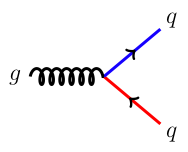
\includegraphics[scale=1]{quarkgluevertex.png}
\caption{Quark quark gluon etkileşimi}
\label{fig:quark}
\end{figure}
İki kuark arasındaki kuvvet en düşük mertebede Şekil \ref{fig:etkilesim} ile belirlenir.
\begin{figure}[!htbp]
\centering
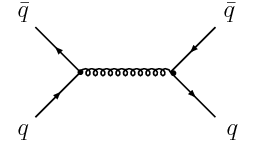
\includegraphics[scale=0.5]{qbarq-qbarq-scattering.png}
\caption{İki kuark arasındaki en düşük mertebeli etkileşim}
\label{fig:etkilesim}
\end{figure}
İki kuark arasındaki kuvvetin qluonların değiş-tokuşu ile taşındığı söylenebilir.
\par Bu düzeyde KRD, KED'e çok benzemektedir. Ancak önemli farklar da vardır. KED de tek bir elektrik yükü varken KRD'de $3$ çeşit rengin bulunmasıdır. $q \rightarrow q + g $ temel sürecinde kuarkın rengi değişebilir (fakat çeşnileri değişmez). Örneğin bir mavi yukarı-kuark, bir kırmızı yukarı-kuarka dönüşebilir. Renk Yükü her zaman korunur; bu, aradaki farklı gluonun taşıdığı anlamına gelir. Şekil \ref{fig:quark} da görüldüğü üzere kuarkların reklerinin biri mavi diğeri kırmızı olabilir bu durumda qluonun rengi $m , \overline{k}$ dır ve renk yükü korunmuş olur. Böylece qluonun iki renkli olduğu anlaşılmaktadır.
\par Gluonların kendileri renk taşıdıkları için doğrudan diğer gluonlarla etkileşmeye girerler, dolayasıyla ilkel kuark-gluon köşesinde ilave olarak ilkel gluon-gluon köşesi vardır.
\begin{figure}[!htbp]
\centering

\includegraphics[scale=1]{WorldOfGlue.png}
\caption{İki çeşit gluon etkileşmesi; 3 gluon köşesi ve dörk gluon köşesi}
\end{figure}
Bu doğrudan gluon-gluon çiftlenimi, KRD'ni KED`e göre daha karmaşık fakat aynı zamanda çok daha zengin kılar.
\par Renk dinamiği ile elektrodinamiği arasında diğer bir fark da çiftlenim sabitinin büyüklüğüdür. KED`ğinde her köşe, hesaba $\alpha =1/137$ faktörü katar. Bu sayının küçük olmasının anlamı, sadece az sayıda köşeye sahip Feynman diyagramlarını göz önüne almamızın yeterli olmasıdır. Güçlü kuvvetler için karşılık gelen çiftlein sabiti $\alpha_s$ 1 den büyük olduğu deneysel olarak gösterilmiştir.
\par Daha karmaşık diyagramlar daha çok katkıda bulunmaktadırlar ve KED için çok iyi çalışan Feynman diyagramları bu durumda işe yaramamaktadırlar. Kuantum renk dinamiğinin büyük zaferlerinin birisi, bu kuramda çiftlenim sabiti rolü oynayan sayının aslında bir sabit olmayıp etkileşen parçacıklar arasındaki uzaklığa bağlı olduğunun keşfidir.\footnote{kayan çiftlenim sabiti.} Nükleer fiziğin karakteristiği olan nispeten uzun mesafelerde büyük iken, çok kısa mesafelerde çok küçük değerler alır. Bu olaya Asimptotik özgürlük olarak bilinir. Asimptotik özgürlük daha net bir deyişle bir proton veya bir pionun içinde kuarkların birbirleriyle fazla etkileşmeden bir arada durmasıdır. Bu davranış deneysel olarak derin esnek olmaya saçılma deneylerinde gözlenmiştir. Kuramsal bakış açısından, asimptotik özgürlüğün keşfedilmesi, yüksek enerjide Feynman cebrinin KRD için geçerli hesaplama aracı olmasını sağlamıştır.

\begin{figure}[!htbp]
\centering
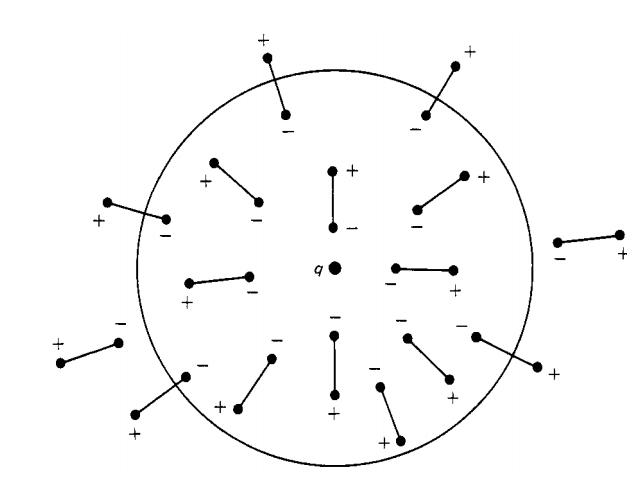
\includegraphics[scale=0.4]{qyuku.png}
\caption{dielektrik bir ortamda bir q yükünün perdelenmesi}
\label{fig:qyuku}
\end{figure}
\par Elektrodinamikte etkin çiftlenim sabiti, kaynaktan olan uzaklığımıza bağlıdır. Bu, nicel olarak şu şekilde anlaşılabilir. İlk olarak bir dielektrik ortam içinde gömülü bir pozitif noktasal q yükünü göz önüne alalım. Şekil \ref{fig:qyuku} 'de gösterildiği gibi, her moleküler dipolün negatif ucu q`ya doğru çekilir ve pozitif ucu uzağa itilir. Sonuç olarak parçacık etrafında, alanı kısmen iptal eden negatif yüklerden oluşan bir kaplama oluşur. Dolayısı ile dielektrik ortamın varlığında, herhangi bir parçacığın etkin yükü bir miktar indirgenir. Tabii ki en yakın molekülden daha yakındaysanız perdeleme yoktur ve q yükünün tümünü görürsünüz.Etkin yük çok küçük uzaklıklarda artmış olur.
\par Kuantum elektrodinamiğinde vakımın kendisi tıpkı bir dielektrik madde gibi davranır. Şekil \ref{fig:feyndiyagram} da gösterildiği gibi pozitron-elektron çiftleri oluşturur.
\begin{figure}[!htbp]
\centering
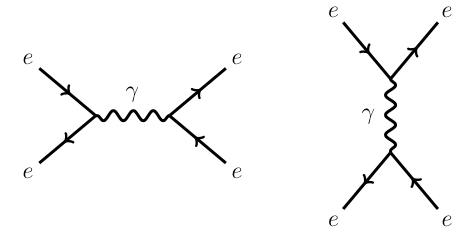
\includegraphics[scale=0.8]{feyndiyagram.png}
\caption{elektron pozitron çiftleri}
\label{fig:feyndiyagram}
\end{figure}

\par Halka sanal elektron q'ya doğru çekilir ve sana pozitron uzağa itilir bu şekilde ortaya çıkan vakum kutuplanması yükü kısmen perdeler ve alanı azaltır. Bir kez daha q yüküne çok yaklaşılırsa perdeleme kaybolur. Her zaman elektron yükü olarak adlandırdığımız büyüklük aslında tümüyle perdelenmiş etkin yüktür. KED`ğindeki durum böyledir. Aynı durum KRD'de de söz konusudur.kuark-kuark-gluon köşesinin yanı sıra şimdi doğrudan gluon-gluon köşeleride vardır.KED`deki vakum kutuplanabilirliğine benzeyen diyagramlara ek olarak şimdi gluon halkalarının da hesaba katmalıyız.
\begin{figure}[!htbp]
\centering
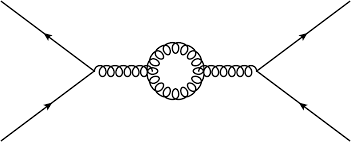
\includegraphics[scale=0.5]{gluonloop.png}
\caption{Gluon loop a sahip bir feynman diyagramı}
\label{fig:gluonloop}
\end{figure}
kuark kutuplanma diyagramları (bunlar kısa mesafelerde $\alpha_s$'yi yukarıya çeker) ile gluon kutuplanması (bunlar ise aşağıya çeker) arasında bir çeşit yarış vardır.

\begin{equation}
a\equiv 2f - 11 n
\end{equation}
Bu sayı pozitif ise, KED`de olduğu gibi etkin çiftlenim kısa mesafelerde artar; negatif ise azalır. Standart Model'de $f=6$ ve $n=3$ ve $a=-21$'dir ve KRD çiftlenimi kısamesafelerde azalır. Asimptotik özgürlüğün kaynağı budur.

\section{Zayıf Etkileşmeler}
elektriksel yükün elektromanyetik kuvvetleri ve renk yükünün güçlü kuvveti üretmesi anlamında zayıf kuvvetleri üreten şeyin özel bir adı yoktur.Tüm kuarklar ve leptonlar bu yükü taşımaktadırlar. İki tür zayıf etkileşme söz konusudur. Bunlar yüklü etkileşmeler (W ların aracılık yaptığı) ve yüksüz etkileşmelerdir(Z'nin aracılık yaptığı).
\subsection{Yüksüz Zayıf Etkileşim}
Z bozonu nötrino-proton saçılması gibi süreçlere aracılık eder.
\begin{figure}[!htbp]
\centering
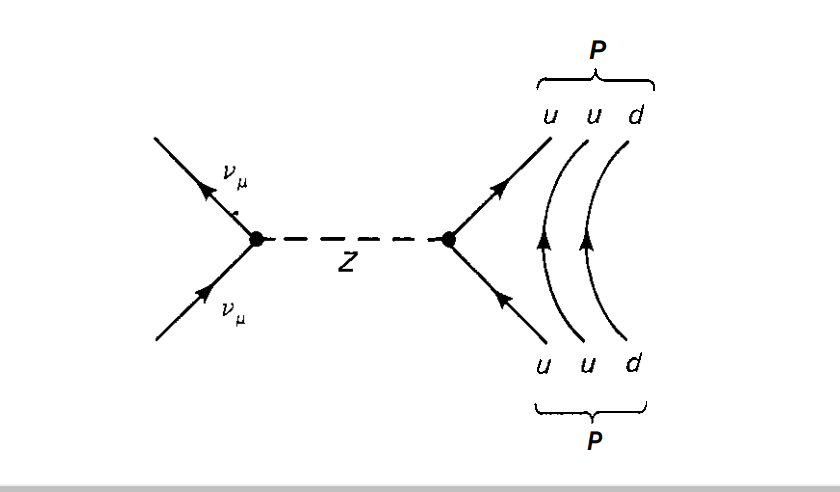
\includegraphics[scale=0.3]{yuksuzZ.png}
\caption{yüksüz etkileşim örneği olarak feynman diyagramı}
\end{figure}
Son durum da,d'ye güçlü kuvvetlerle (gluon değiş tokuşu) bağlı olan  iki seyirci kuark aktif rol oynamadan olaya katılır. Bir fotonun aracılık ettiği herhangi bir sürece Z'nin de aracılık edebilebilir. Coulomb yasasına ikinci diyagramdan gelen bir düzeltme vardır fakat fotonun aracılık yaptığı süreç çok baskındır. Atom fiziğinde, elektromanyetik süreçlerdeki yüksüz zayıf kirlilik zayıf etkileşmelerin taşıdığı parmak izinden yararlanılarak ayırt edilebilir. Katkının çok küçük olmasından dolayı nötrino deneyleri oldukça zordur.
\subsection{Yüklü Zayıf Etkileşim}
İlkel köşelerin güçlü, elektromanyetik ve yüksüz zayıf etkileşimler için paylaşıldığı özellik, çıkan kuark veya leptonun gelen ile aynı olmasıdır. KRD'de kuarkların rengi değişebilir ama çeşni hiçbir zaman değişmez. Çeşniyi değiştiren sadece yüklü zayıf etkileşmelerdir.
\subsubsection{Leptonların Yüklü Zayıf Etkileşimi}
Bir negatif yüklü lepton bir $W^-$ yayımlayarak buna karşılık gelen bir nötrinoya dönüşür. 
\begin{figure}[!htpb]
\centering
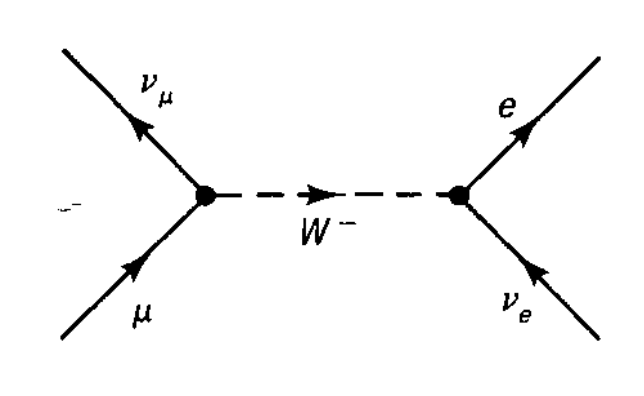
\includegraphics[scale=0.3]{leptonlar.png}
\caption{Leptonik bozunum}
\end{figure}


\subsection{Kuarkların Etkileşimi}
Bu kuram da elektron sayısı, müon sayısı ve tau sayısının korunumu şattır. Şekil \ref{fig:cesnidegis} 'de $-1/3$ yüklü bir kuark bir $W^-$ bozonu yayımlayarak $+2/3$ yüklü bir kuarka dönüşür. Çıkan kuark gelen kuarkla ayrı rengi taşır, ama çeşnisi değişmiştir.

\begin{figure}[!htpb]
\centering
\begin{subfigure}{.5\textwidth}
  \centering
  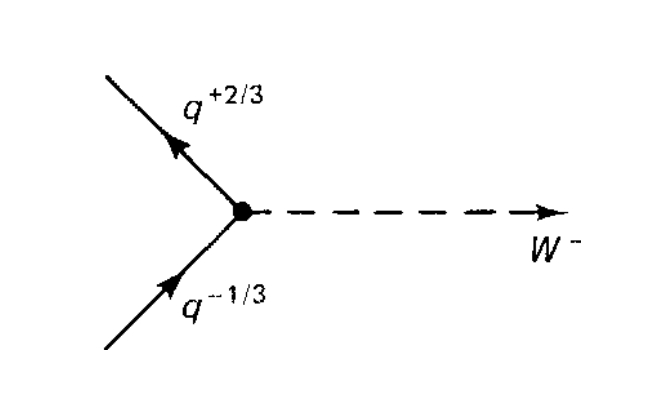
\includegraphics[width=.8\linewidth]{cesnidegis.png}
  \caption{$W^-$ ozunumuyla çeşni değiştiren quarklar}
  \label{fig:cesnidegis}
\end{subfigure}%
\begin{subfigure}{.5\textwidth}
  \centering
  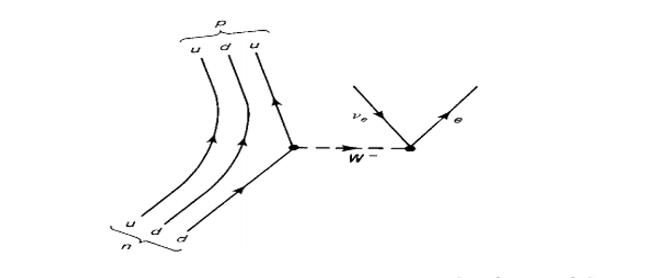
\includegraphics[width=.8\linewidth]{protonnotron.png}
  \caption{Nötronun beta bozunumu}
  \label{fig:sub2}
\end{subfigure}
\caption{Kuark etkileşmesi}
\label{fig:test}
\end{figure}

Bu etkileşim ile temelde nötronun beta bozunumunu da gösterebiliriz.

\subsection{Bozunumlar ve Korunum Yasaları}
Temel parçacıkların en genel özelliklerinden birisi parçalanmaya olan eğilimleridir. Bu durumu evrensel bir ilke şeklinde ifade edebiliriz. Bir korunum yasası tarafından engellenmediği sürece, her parçacık kendisinden daha hafif parçacıklara bozunur.
\begin{table}[!htpb]

\centering
\begin{tabular}{|c|c|c|}
\hline 
foton & kararlı & kütlesiz \\ 
\hline 
elektron & kararlı & en hafif yüklü parçacık \\ 
\hline 
proton & kararlı & en hafif baryon \\ 
\hline 
\end{tabular}
\caption{bazı parçacıkların kararlılıkları ve sebebleri}
\end{table}
Tablo  da açıkça görüldüğü üzere yük korunumu ve baryon korunumu için bu temel parçacıklar için kararlı diyebiliyoruz.Fakat çoğu parçacık (birçok atom çekirdeğinin koruyucu ortamında kararlı olmakla birlikte nötron bile) kendiliğinden bozunur.Çevremizde esas olarak protonlar, nötronlar, elektronlar, fotonlar ve nötrinolar bulunmaktadır. Daha egzotik parçacıklar zaman zaman çarpışmalarda üretilirler ama fazla yaşamazlar.Her kararsız türün bir karakteristik ömrü $\tau$ vardır. Parçacıkların çoğu birkaç farklı bozunum moduna sahiptir, örneğin $K^+$ ların $\%64$ ü $(\mu^+ + v_\mu )$ şeklinde bozunurken, $\%21$'i $(\pi^+ + \pi^0)$'a $\%6$'sı $(\pi^+ + \pi^+ + \pi^- )$'ye ve $\%5$'i ise $(e^+ + v_e + \pi^0)$'a bozunmaktadır. Temel parçacık kuramının hedeflerinden birisi de bu ömür ve dallanma oranlarının hesaplanmasıdır. 
\par Verilen bir bozunum üç temel kuvvetten birisi tarafından meydana getirilir. Bunlar güçlü, elektromanyetik ve ya zayıf boozunumlardır.

\begin{table}[!htpb]
\centering
\begin{tabular}{|c|c|}
\hline 
Bozunum & Bozunum Türü \\ 
\hline 
$\triangle^{++} \rightarrow p^+ + \pi^+$ & Güçlü  \\ 
\hline 
$\pi^0 \rightarrow \gamma + \gamma$ & Elektromanyetik \\ 
\hline 
$\sum^- \rightarrow n + e^- + \overline{v_e} $ & Zayıf \\ 
\hline 
\end{tabular} 

\caption{Bozunumlar ve Bozunum Türleri}
\end{table}
Eğer bozunumda bir foton çıkıyorsa süreç mutlaka elektromanyetik, nötrino çıkıyorsa mutlaka zayıftır. Ancak bunlar çıkmadığında ne olduğunu söylemek oldukça zordur. Güçlü bozunumun ömrü $10^{-23}s$ civarında, elektromanyetik bozunum  $10^{-16}s$ ve zayıf bozunum $10^{-13}s$'den 15 dakikaya kadar değişebilir.Bozunum genellikle ana parçacık ile ürün parçacık arasındaki kütle farkıyla ters orantılıdır.  

\begin{figure}[!htpb]
\centering
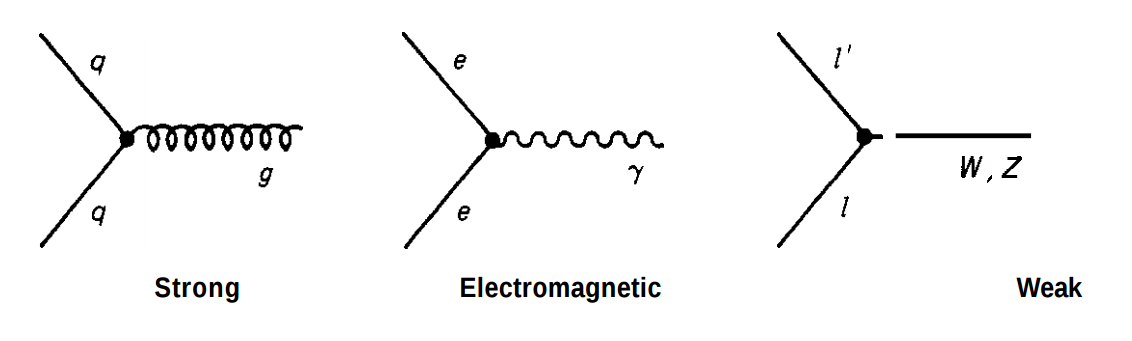
\includegraphics[scale=0.4]{bozunumkurallari.png}
\caption{üç bozunum türü için Feynman diyagramları}
\end{figure}
Tüm fiziksel süreçleri temel diyagramları karmaşık kombinasyonlar halinde bir araya getirerek elde etmek mümkün olduğundan dolayı, her köşe için tepkimenin tamamında korunmalıdır. Korunma yasaları;

\begin{enumerate}
\item \emph{Yük : } 
\par Her üç etkileşmedede elektrik yükünü korur. Zayıf etkileşmelerde yük farkı olabilir ve bu farkı W taşır.
\item \emph{Renk : }
\par Elektromanyetik ve zayıf etkilşmelerde renk etkilenmez. Bir güçlü etkileşim köşesinde kuark rengi değişir, farkı gluon taşır.Doğada bulunan parçacıklar renksiz olduğundan korunumun gözlenmesi çok kaydır. Tepkimeye giren renk sıfır ve tepkimeden çıkan renk sıfır olmalıdır.

\item \emph{Baryon Sayısı : }
\par Bütün ilkel köşelerde, eğer bir kuark girerse, bir kuark da çıkar ve dolayısı ile mevcut kuark sayısı sabittir. Bu işlem de antikuarklar negatif sayılır.

\item \emph{Lepton Sayısı : }
\par Güçlü kuvvetler hiç bir şekilde leptonlara dokunmaz; bir elektromanyetik etkileşmede giren lepton aynen çıkar.

\item \emph{Çeşni : }
\par Çeşni güçlü ve elektromanyetik köşelerde korunur ancak zayıf etkileşim köşelerinde korunmaz.Yani bir yukarı kuark bir aşağı-kuark veya acayip kuarka dönüşebilir.Kaybedilen yukarılığı taşıyan veya kazanılan aşağılığı veya acayipliği sağlayan birşey yoktur. Zayıf kuvvetler çok zayıf olduğundan değişik çeşnilerin yaklaşık olarak korunduğunu söyleriz.

\end{enumerate}

\section{CMS (Compact Muon Solenoid)}
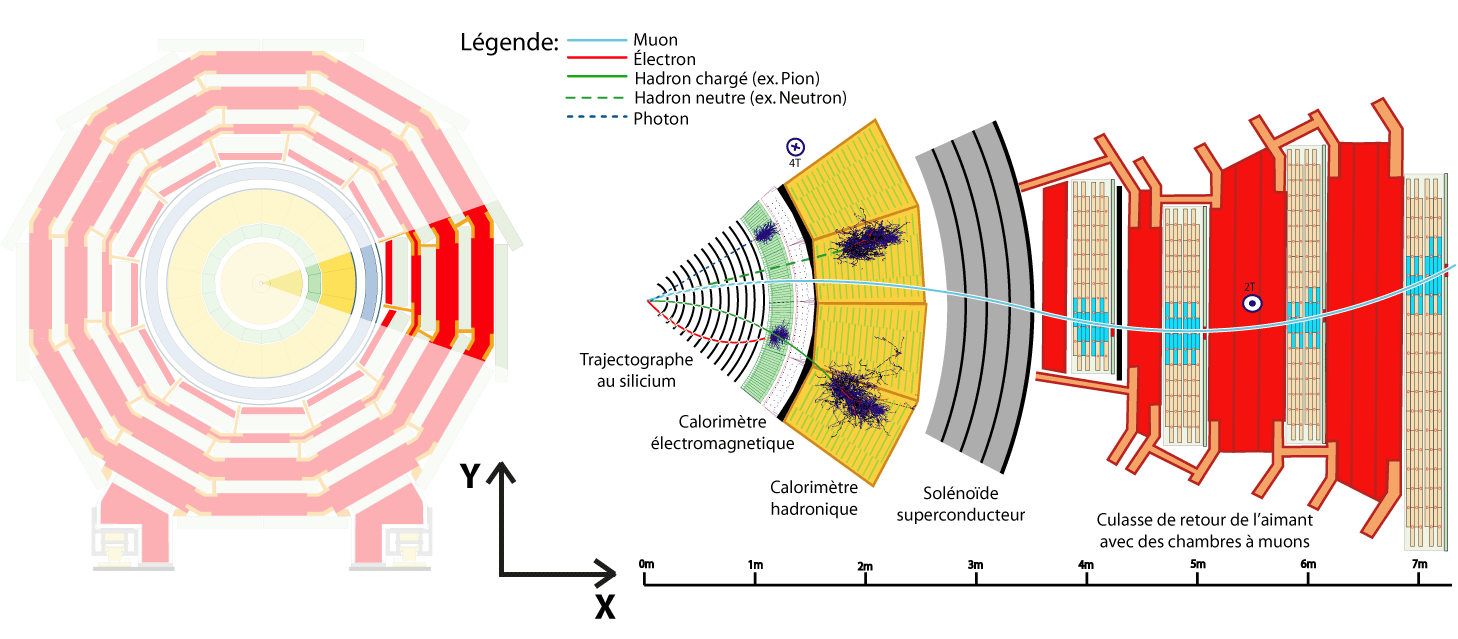
\includegraphics[scale=0.2]{slice_white_v1}
\subsection{CMS Dedektörü Şeması}
\newpage

\subsection{CMS Teorik Bilgi}



\begin{align}
desdsdasdb=sdab s \\
\eta = -ln(\cos \theta /2)
\end{align}







\newpage
\subsubsection{Kinematik Değişkenler}
\subsubsection*{Kayıp Enerji (Missing $E_t$)}
\subsubsection*{Muon}
\subsubsection*{Elektron}
\subsubsection*{$P_t$}
\subsubsection*{$\eta$}
\subsubsection*{$\phi$}

\chapter{Monte Carlo Simülasyonu ve Data Üretimi}
\section{Monte Carlo Simülasyonu}
Rastgele üretilen sayılardan daydalanılarak istatistiksel simülasyonlar Monte Carlo (MC)\footnote{Los Alamos Bilimsel Laboratuar’ından John Von Neumann, Stan Ulam ve Nick Metropolis adlarında üç bilim adamı tarafından ortaya çıkarılmıştır. Metropolis algoritması olarak da bilinir.} metoduyla yapılır. 
Deney girdileri belirli olmayan, kesin olmayan bir sekilde gelmesi bekleniyorsa ve dağılım bir fonksiyonla hesaplanabilecekse kullanılır. MC, rastgele sayıları baz alarak tahmini sistemleri modeller. MC methodunun kullanıldığı bazı alanlar, Sayisal Analiz, Atom ve Molekul Fiziği, Nükleer Fizik, Yüksek Enerji Fiziği gibi alanlarda modellerle test edilebilen simulasyonlar gerçekleştirilir. 
\par 1930 yılında İtalyan bir fizikçi olan Enrico Fermi’nin, yeni keşfedilmiş olan nötronun özelliklerinin hesaplaması sırasında Monte Carlo Yöntemi’ni kullanması ile bu yöntemin adı duyulmuş oldu. Sınırlı hesaplama kaynaklarına sahip olunduğunda sıklıkla kullanılan bir yöntemdir. Örnek olarak Monte Carlo Yöntemi İkinci Dünya Savaşı sırasında ilk atom bombasının geliştirildiği Manhattan Projesi’nde kullanılmıştır. MC yönteminde yüksek boyutlu integrallerin çözümünü daha kolaylaştırmakta ve hata oranı işlem yapılmadan önce yaklaşık olarak rahatlıkla kestirilebilmektedir  
\begin{equation}
I= \int_{x_1}^{x_2} f(x) dx \equiv (x_2 - x_1) \frac{1}{N}\sum_{i=1}^N f(x_i)
\end{equation}
\par $x= (x^1,x^2,\cdots ,x^d)$, $d$ integral boyutunu göstermek üzere, integrali toplam şeklinde gösterimi:
\begin{equation}
I=\int_R f(x) dx = \triangle x^d \sum_{i_1 =1}^N \sum_{i_2 =1}^N \cdots \sum_{i_d =1}^N f(x_{i_1}^1,\cdots,x_{i_d}^d)
\end{equation}
şeklinde ifade edebiliriz. Her bir boyut için 10 adet örnek eleman kullandığımızda yapmamız gereken işlem sayısı $N^d =10^5=100000$ dir. MC için hata oranı $\left(\frac{1}{\sqrt{N}}=\frac{1}{\sqrt{100000}}=0.00316 \right)$ dir.
\par \textbf{\textit{MC yöntemine ait bir kaç teknik mevcuttur.}}
\par \textbf{Reddetme yöntemi: \footnote{Rejetion Method} } Sekil \ref{fig:reject} seçilen rastgele noktalar eğer $f(x)$ fonksiyonuna ait eğrinin altında kalıyorsa kabul, değilse reddedilerek toplam yapılan denemelerden kaç tanesinin başarılı sonuç verdiği hesaplanır. Yapılan işlemler sonucunda, toplam deneme sayısının başarılı deneme sayısına oranı, toplam alanın integrali alanın integrali alınarak istenilen $f(x)$ fonksiyonunun alanına oranını verir.
\par Bu yöntem bir veya daha fazla keskin tepe noktası olan fonksiyonlar için uygun bir yontem değildir. Reddedilen noktalar vakit kaybına sebeb olur şekil \ref{fig:reject2}

%%%%%%%%%%%%%%%%%%%%%%%%%%%%%%%%%%%%%%%%%%%%%%%%%%%%
\begin{figure}[!htpb]
        \centering
        \begin{subfigure}[b]{0.35\textwidth}
            \centering
            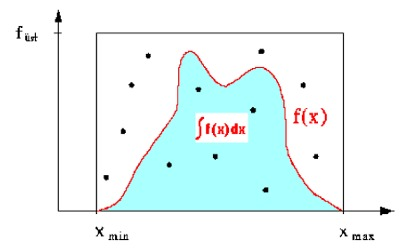
\includegraphics[width=\textwidth]{reject}
            \caption[Reddetme yontemi]%
            {{\small Reddetme yontemi}}    
            \label{fig:reject}
        \end{subfigure}
        \hfill
        \begin{subfigure}[b]{0.35\textwidth}  
            \centering 
            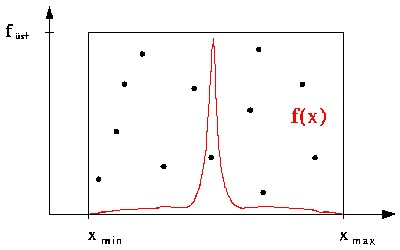
\includegraphics[width=\textwidth]{reject2}
            \caption[keskin tepe noktasina sahi olan fonksiyon]%
            {{\small keskin tepe noktasina sahi olan fonksiyon}}    
            \label{fig:reject2}
        \end{subfigure}
        \vskip\baselineskip
        \begin{subfigure}[b]{0.35\textwidth}   
            \centering 
            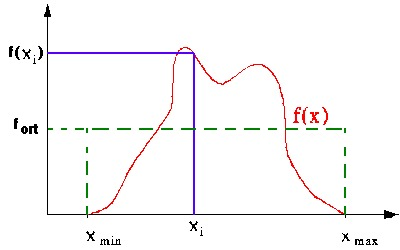
\includegraphics[width=\textwidth]{average_mc}
            \caption[Monte Carlo icin ortalama yontemi]%
            {{\small Monte Carlo icin ortalama yontemi}}    
            \label{fig:avarage}
        \end{subfigure}
        \quad
        \begin{subfigure}[b]{0.35\textwidth}   
            \centering 
            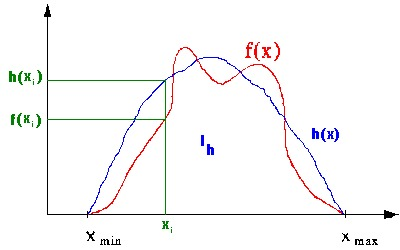
\includegraphics[width=\textwidth]{kontrol}
            \caption[Kontrol Degiskeni Yontemi]%
            {{\small Kontrol Degiskeni Yontemi}}    
            \label{fig:kontrol}
        \end{subfigure}
        \caption[ Monte Carlo Yontemleri]
        {\small Monte Carlo Yontemleri} 
        \label{fig:MonteCarlo}
    \end{figure}

%%%%%%%%%%%%%%%%%%%%%%%%%%%%%%%%%%%%%%%%%%%%%%%%%%%%

\par \textbf{Ortalama Yöntemi : \footnote{Averaging Method}} Şekil \ref{fig:avarage} görüldüğü gibi ortalama yöntemide rastgele seçilen noktalar üzerinden işlem yapar. Reddetme yönteminden farklı olarak, alan taramak yerine, seçilen noktalardaki fonksiyonun değerinden yola çıkarak sonucu bulmaya çalışır.


\par \textbf{Kontrol Değişkeni Yöntemi : \footnote{Control Variates Method}} Bu yöntemde, integrali alınmak istenen $f(x)$ fonksiyonuna oldukça yakın bir $h(x)$ yardımcı fonksiyonu kullanılır. Bu yardımcı fonksiyonun integral değeri, $f(x)$ fonksiyonumuzdan daha kolay hesaplanabilir veya çözümü bilinen bir fonksiyon olmalıdır .Böylelikle seçilen her rastgele noktada iki fonksiyonun farkından, integral değerleri arasındaki fark bulunmaya çalışılır. Elde edilen fark değeri $h(x)$ fonksiyonunun integral değerine eklenerek $f(x)$ fonksiyonuna ulaşılmaya çalışılır. \ref{fig:kontrol}


\begin{equation}
\begin{aligned}
\textbf{ Monte Carlo } \varpropto \frac{1}{\sqrt{N}}\\
\textbf{Trapezium } \varpropto \frac{1}{N^{\frac{2}{d}}}\\
\textbf{Simpson's } \varpropto \frac{1}{N^{\frac{4}{d}}}\\
\end{aligned}
\end{equation}
\par Yukarıda görüldüğü uzere Monte Carlo metodu diğer yöntemlere göre integralin boyutuna bağlı değildir. Bu yüzden MC yönteminde eğer tek katlı integral çözümü yapılacaksa zaman alabilir ancak çok katlı integrallerde MC yöntemi integralin boyutundan bağımsız olduğu için açık ara bir avantaj sağlayacaktır.

\par Matematikte ve fizikte bir faz uzayı içinde bir sistemin tüm olası durumlarının temsil edildiği bir uzaydır. Sistemin her olası durumuna karşılık faz uzayında bir tek nokta vardır. Parçacık çarpışma işleminde teorik olarak çok katlı integrallerin çözümleri gerekmektedir. Eğer son durumda $n$ adet parçacık varsa $d=3 n - 4 $ adet faz uzayı mevcuttur. 2 parçacığın çarpışıp 3,4,...,n parçacıklarını ürettiklerini varsayalım:
\begin{equation}
1+2 \rightarrow 3 + 4 + ... + n
\end{equation}
\par Sacılma tesir kesiti,
\begin{equation}
\begin{aligned}
\sigma=  \frac{S \hbar^2}{4\sqrt{(p_1 \cdot p_2)^2 - (m_1 m_2 c^2)^2}}\int |\mathscr{M}|^2 (2 \pi)^4 \delta^4(p_1 + p_2 - p_3 \cdots - p_n) \\ \times \prod_{j=3}^n \frac{1}{2\sqrt{\textbf{p}_j^2+m_j^2c^2}}\frac{d^3 \textbf{p}_j}{(2\pi)^3} 
 \end{aligned}
\end{equation}
dormülü ile verilir. Burada $p_i$ $i$. parçacığın 4-vektör momentumudur (kütlesi $m_i$) ve $S$ istatistiksel düzeltme faktörüdür. Örnek olarak, $a \rightarrow b + b +c +c +c$ gibi bir sureç için $S= (1/2!)(1/3!)=1/12$ olur. $\mathscr{M}$ ise genliği belirtmektedir\footnote{$\mathscr{M}$ nin nasıl elde edileceği Ekler Kısmında Bir Oyuncak Kuram İçin Feynman kurallarında anlatılmıştır}.

\section{Olay Üretimi}
\subsection{MadGraph}
MadGraph\footnote{MadGraph'in ilk versiyonu Fortran'da 1994 yılımda  Tim Stelzer tarafından yazılmıştır.} programı yüksek enerji fiziğinde parçacık çarpıştırmasında parçacıkların son durumlarını veren ve MC metodunu kullanan bir similasyon yazılımıdır.Ağaç seviyesinde matrix elemanı hesaplayıcısı, tesir kesiti hesabı ve olay üretimi yapan MG uzun süre C++/Fortran ile hazırlanan MG4, 2010 yılından bu yana Python dilinde hazırlanan MG5 i kullanmaktadır. MG5 Grid üzerinde, çok çekirdekli ya da küme bilgisayarlarda başarılı hesaplamalar yapabilmektedir. 
\begin{figure}[!htpb]
\centering
	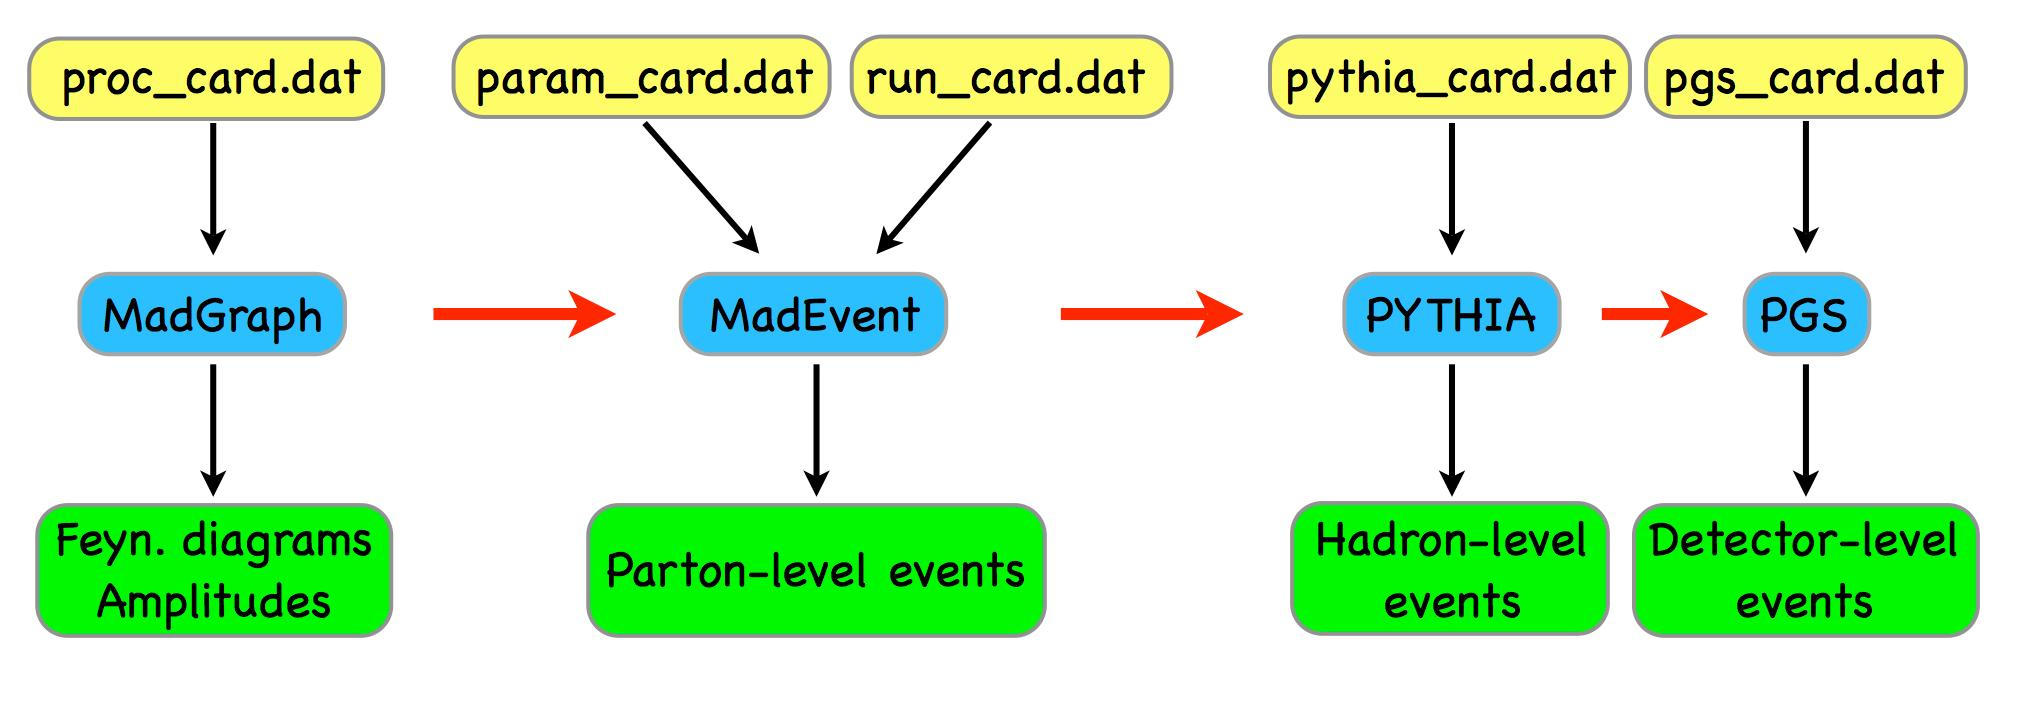
\includegraphics[scale=0.2]{madgraphwork}
	\caption{MadGraph programının çalışma şeması}
	\label{fig:mgwork}
\end{figure}

Şekil \ref{fig:mgterminal} de görüldüğü üzere kullanıcı arayüzü yoktur. Terminal üzerinden çalıştırılır. Sonuçları HTML olarak verir.


\begin{figure}[!htpb]
\centering
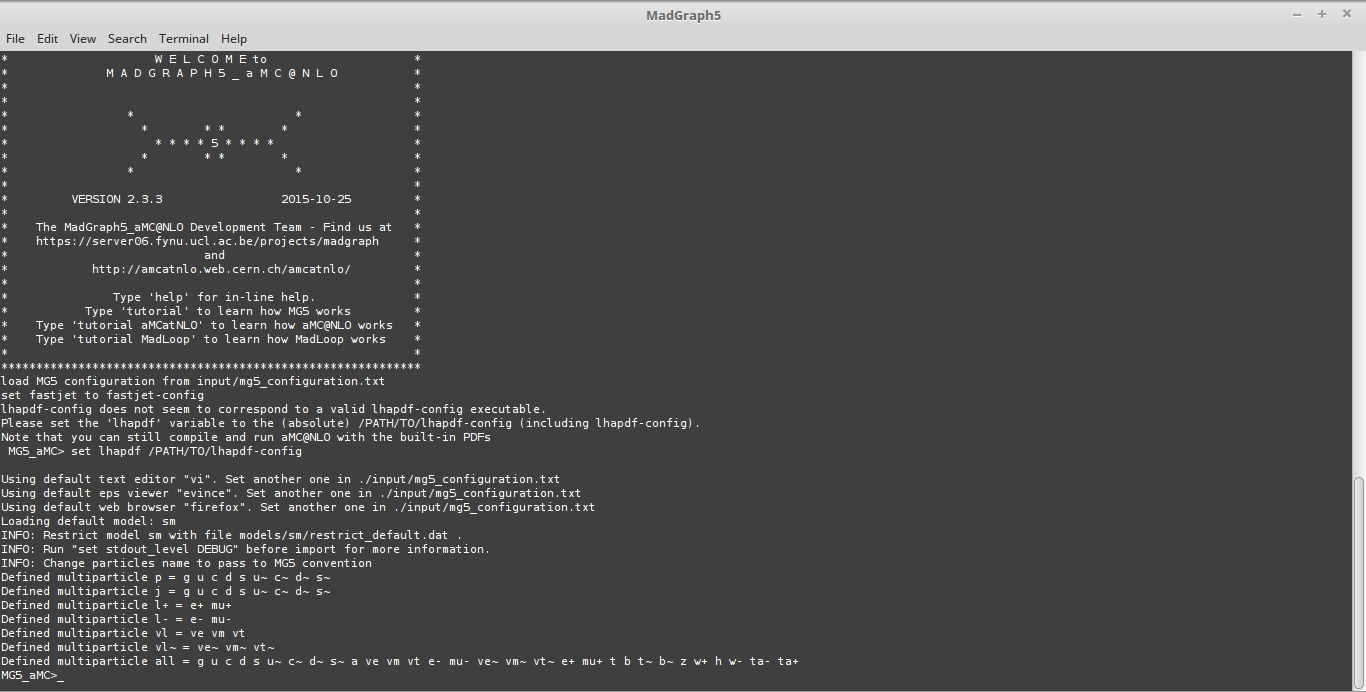
\includegraphics[scale=0.3]{madgraph5}
\caption{MadGraph programının teminal üzerinde görüntüsü}
\label{fig:mgterminal}
\end{figure}


MadGraph programı açık kaynak koddur ve kurulumu bir kaç basit adımda gerçekleştirilebilir\footnote{Ekler kısmında MadGraph kurulumu anlatılmıştır.}. MG çalışma prensibi ve çalışma adımları. 


\par \textbf{MadGraph : } 
\par MadGraph da olay üretimi için $proc\_card.dat$ dosyasını kullanır.

\begin{lstlisting}
import model sm-no_b_mass
define p = g u c d u~ c~ d~ s~
generate p p > j j
output 100-250
\end{lstlisting}
\texttt{ import model }satırında kullanmak istediğimiz modelimizi tanımlıyoruz. Daha sonra parçacıkların ne içerdiğini  \texttt{define} ile belirtiyoruz. \texttt{generate} komutu ile istediğimiz olayı tanımlayıp olay üretimimizi başlatabiliriz. Olay üretimi başladıktan sonra MG ilk olarak istenilen Feynman diyagramlarını çıkartıyor. 

\begin{figure}[!htpb]
\centering
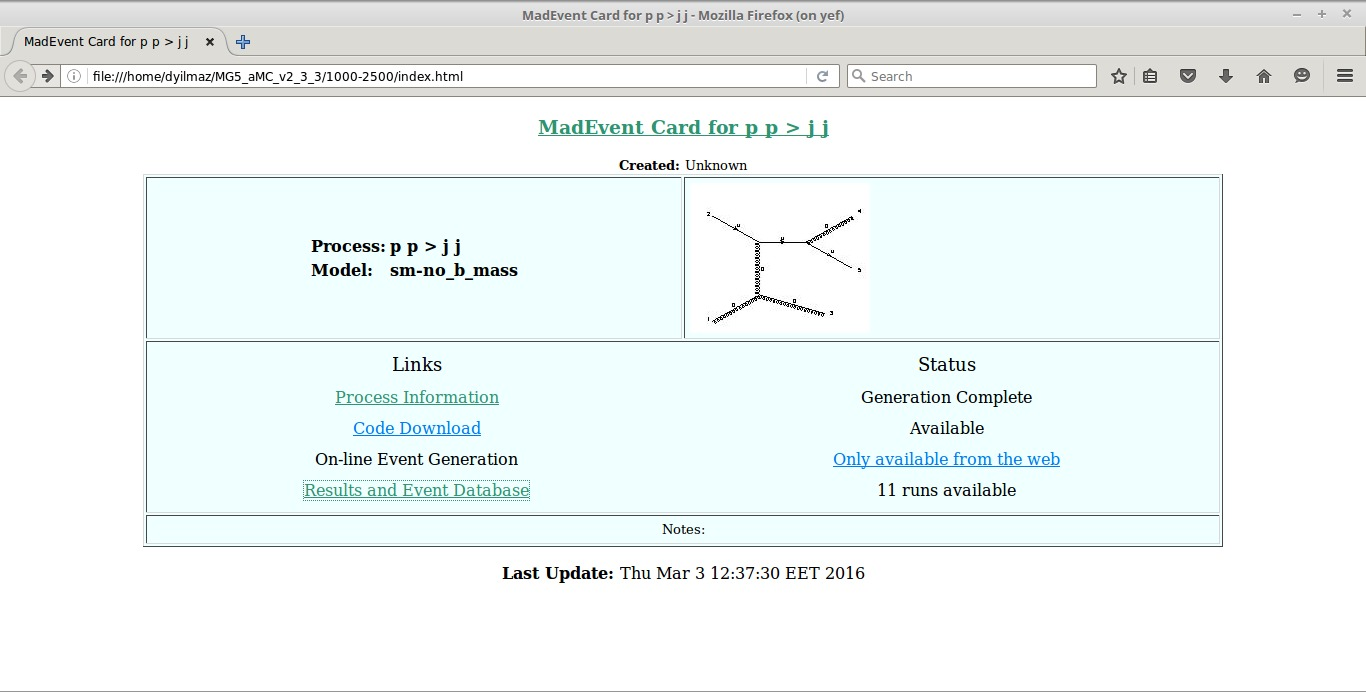
\includegraphics[scale=0.3]{madgraphsecreen}
\caption{MadGraph programının analiz sonucu HTML çıktısı}
\label{fig:mgscreen}
\end{figure}

\par \textbf{MadGraph Feynman Diyagramları Üretimi}\footnote{Anlatılan kartların içeriği Ekler kısmında mevcuttur.}
MG içerisinde $proc\_card.dat$ dosyasında kullandığımız model \texttt{models} adlı klasörde kullandığımız model\footnote{Biz olay üretimimizde sm-no\_b\_mass kullandık} klasöründe; parçacık bilgilerini, köşegen bilgilerini ve diğer bilgileri kullanarak Feynman kurallarına uygun Feynman diyagramlarını çıkartıyor. Birkaç örnek olarak;

Kuplaj parametreleri couplings.py dosyasıyla;
\begin{lstlisting}
GC_1 = Coupling(name = 'GC_1',
                value = '-(ee*complex(0,1))/3.',
                order = {'QED':1})
                
GC_44 = Coupling(name = 'GC_44',
                 value = '(CKM2x1*ee*complex(0,1))/(sw*cmath.sqrt(2))',
                 order = {'QED':1})
\end{lstlisting}
Kuplaj sabitlerini belirliyor. Ayrıca köşegenler için ise vertices.py;
\begin{lstlisting}
V_1 = Vertex(name = 'V_1',
             particles = [ P.G0, P.G0, P.G0, P.G0 ],
             color = [ '1' ],
             lorentz = [ L.SSSS1 ],
             couplings = {(0,0):C.GC_33})
             
V_46 = Vertex(name = 'V_46',
              particles = [ P.a, P.W__plus__, P.G__minus__ ],
              color = [ '1' ],
              lorentz = [ L.VVS1 ],
              couplings = {(0,0):C.GC_75})
\end{lstlisting}
ayrıca decays.py;
\begin{lstlisting}
Decay_e__minus__ = Decay(name = 'Decay_e__minus__',
                         particle = P.e__minus__,
                         partial_widths = {(P.W__minus__,P.ve):'((Me**2 - MW**2)*((ee**2*Me**2)/(2.*sw**2) + (ee**2*Me**4)/(2.*MW**2*sw**2) - (ee**2*MW**2)/sw**2))/(32.*cmath.pi*abs(Me)**3)'})
                         
Decay_ta__minus__ = Decay(name = 'Decay_ta__minus__',
                          particle = P.ta__minus__,
                          partial_widths = {(P.W__minus__,P.vt):'((MTA**2 - MW**2)*((ee**2*MTA**2)/(2.*sw**2) + (ee**2*MTA**4)/(2.*MW**2*sw**2) - (ee**2*MW**2)/sw**2))/(32.*cmath.pi*abs(MTA)**3)'})

\end{lstlisting}
elektron anti tau gibi parçacıkların decay bilgilerini tanımlıyor.\\

\par \textbf{MadEvent} 
\par MadEvent kısmında MG programı $param\_card.dat$ ve $run\_card.dat$ dosyaları kullanılarak çıkmış olan Feynman diyagramlarının genlikleri ($\mathscr{M}$), saçılma tesir kesiti gibi hesaplamalar yapılmaktadır.


\begin{lstlisting}
#*********************************************************************
  100000 = nevents ! Number of unweighted events requested
  0   = iseed   ! rnd seed (0=assigned automatically=default))
#*********************************************************************
# Collider type and energy                                           *
# lpp: 0=No PDF, 1=proton, -1=antiproton, 2=photon from proton,      *
#                                         3=photon from electron     *
#*********************************************************************
     1        = lpp1    ! beam 1 type 
     1        = lpp2    ! beam 2 type
     6500.0     = ebeam1  ! beam 1 total energy in GeV
     6500.0     = ebeam2  ! beam 2 total energy in GeV
#*********************************************************************
\end{lstlisting}
 $run\_card.dat$ dosyasından kaç tane olay üreteceğimiz, çarpıştıracağımız parçacıkların neler ve hangi enerjide olduklarını ayarlayabiliyoruz.
\begin{lstlisting}
#*********************************************************************
# Minimum and maximum pt's (for max, -1 means no cut)                *
#*********************************************************************
20.0  = ptj       ! minimum pt for the jets 
-1.0  = ptjmax    ! maximum pt for the jets
0.0 = drjj    ! min distance between jets 
-1.0  = drjjmax ! max distance between jets
30.0   = xqcut   ! minimum kt jet measure between partons
\end{lstlisting}
Arıca çıkacak olan Jet lerin minimum enerjisi maksimum enerjisi aralarındaki minimum ve maximum uzaklık gibi son durumda elde etmek istediğimiz parçıkların veya Jetlerin özelliklerini belirleyebiliyoruz. Bu ayarlamaları yaptıktan sonra MadEvent kısmında saçılma tesir kesiti ve genlik hesabı yapılmaktadır ve yapılan bu hesaplamalara göre istediğimiz son durumlar MC yöntemi kullanılara simüle edilmektedir.
\par Hadron çarpıştırıcısında bir tesir kesiti hesabı ;
\begin{equation}
\sigma =\frac{1}{F} \sum_ab  \int dPS^{(n)} dx_a dx_b f_{(a/p)}(x_a) f_{(b/p)}(x_b) \overline{|M_{fi}|^2}
\end{equation}
tüm partonlar üzerinden toplam alınır. Burada $f$ parton dağılım fonksiyonudur (PDF). a ve b protondan gelen birer parton ve x parton fraksiyonları olmak üzere $f(x)$ partonların protonlardan gelme olasılığını gösterir.

\begin{figure}[!h]
\centering
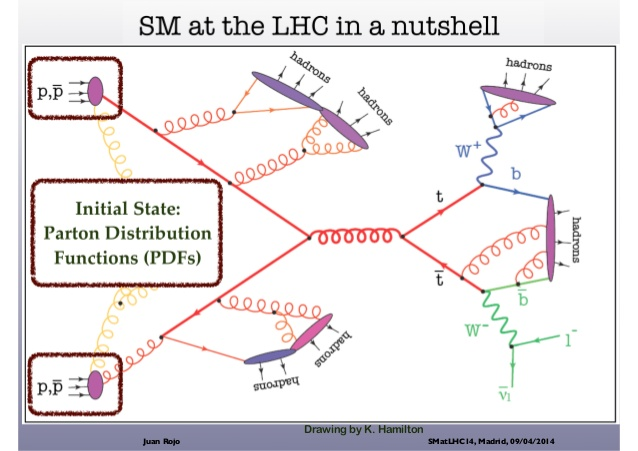
\includegraphics[scale=0.5]{pdf}
\caption{Parton dağılım fonksiyonu ve diğer adımlar}
\label{fig:pdf}
\end{figure}

 Hangi PDF setini kullanacağımızı bu kart içerisinde girebiliriz. Bizim olay üretiminde kullandığımız PDF seti nn23lo1.

\begin{figure}[!htpb]
\centering
\begin{subfigure}[b]{0.5\textwidth}
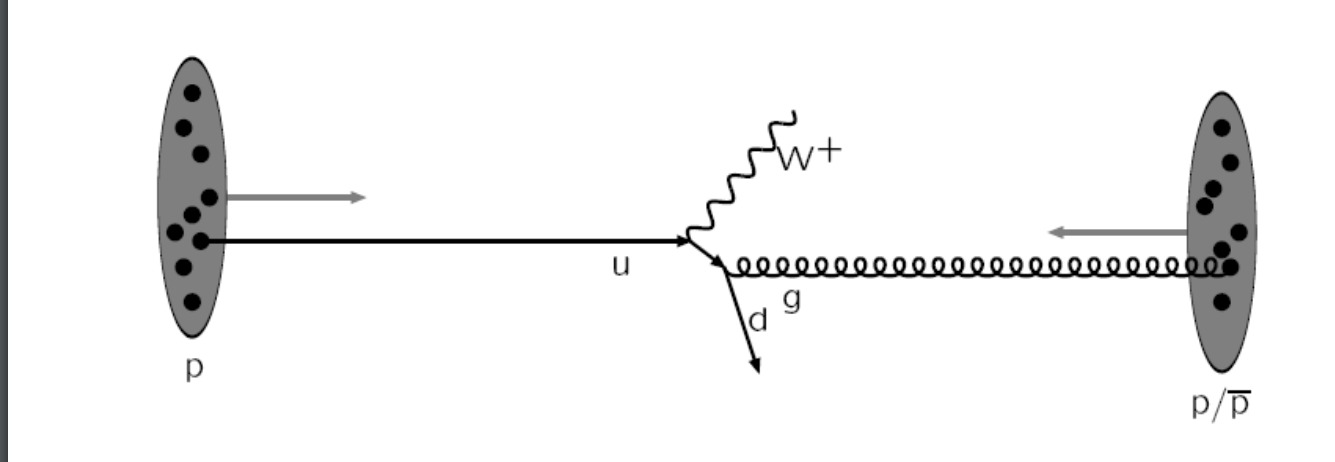
\includegraphics[scale=0.2]{1}
\caption{Sert Saçılma}
\end{subfigure}

\begin{subfigure}[b]{0.5\textwidth}
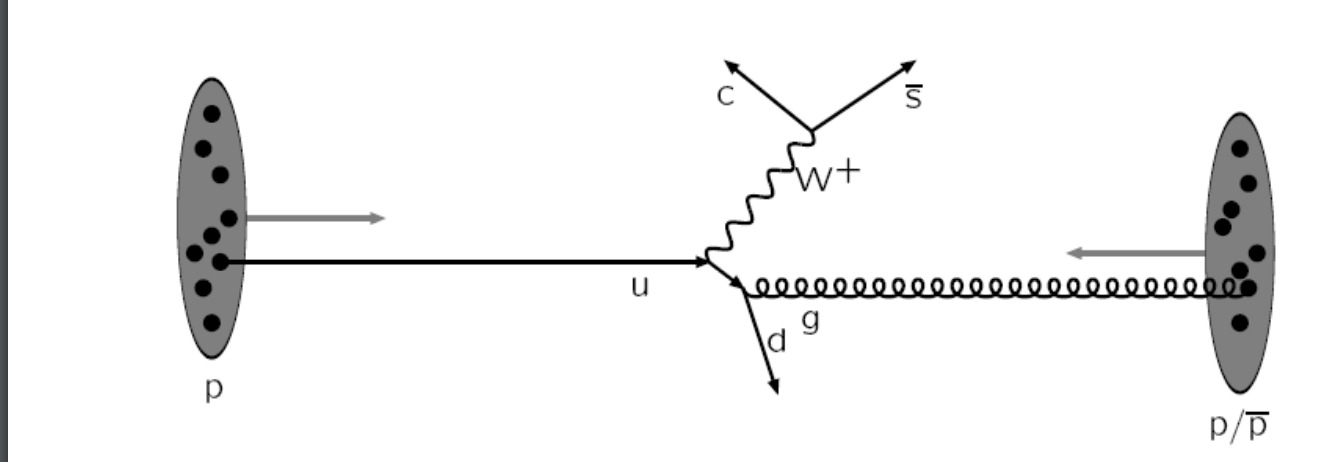
\includegraphics[scale=0.2]{2}
\caption{Alt olay}
\end{subfigure}

\begin{subfigure}[b]{0.5\textwidth}
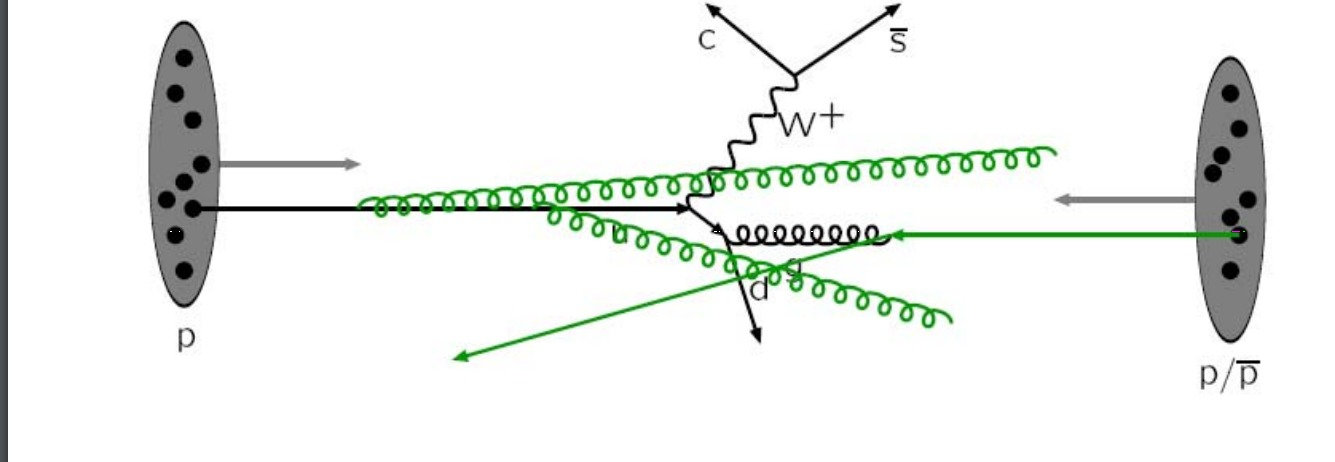
\includegraphics[scale=0.2]{3}
\caption{Başlangıç Durumu Radyasyonu}
\end{subfigure}

\begin{subfigure}[b]{0.5\textwidth}
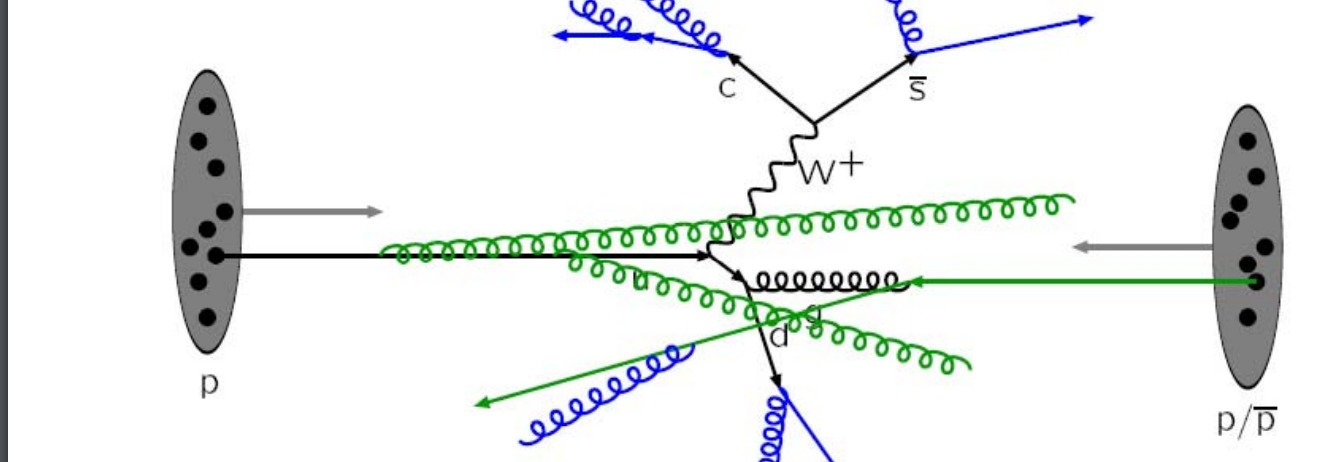
\includegraphics[scale=0.2]{4}
\caption{Son Durum Radyasyonu}
\end{subfigure}

\begin{subfigure}[b]{0.5\textwidth}
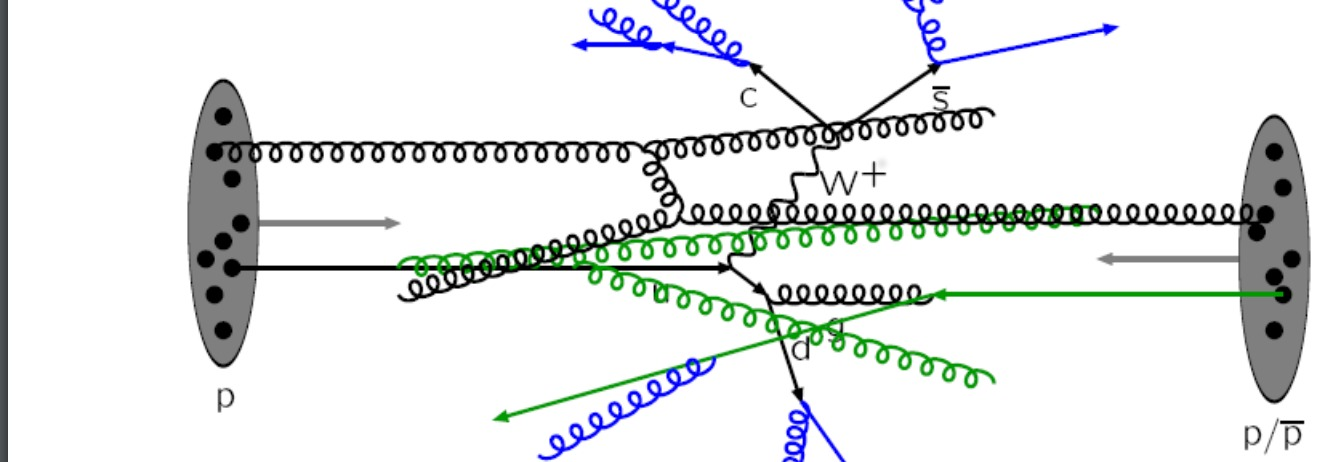
\includegraphics[scale=0.2]{5}
\caption{Çoklu Parton Etkileşimi}
\end{subfigure}
\caption{Proton - Proton Çarpışması adımları}
\end{figure}


\begin{figure}[!h]
		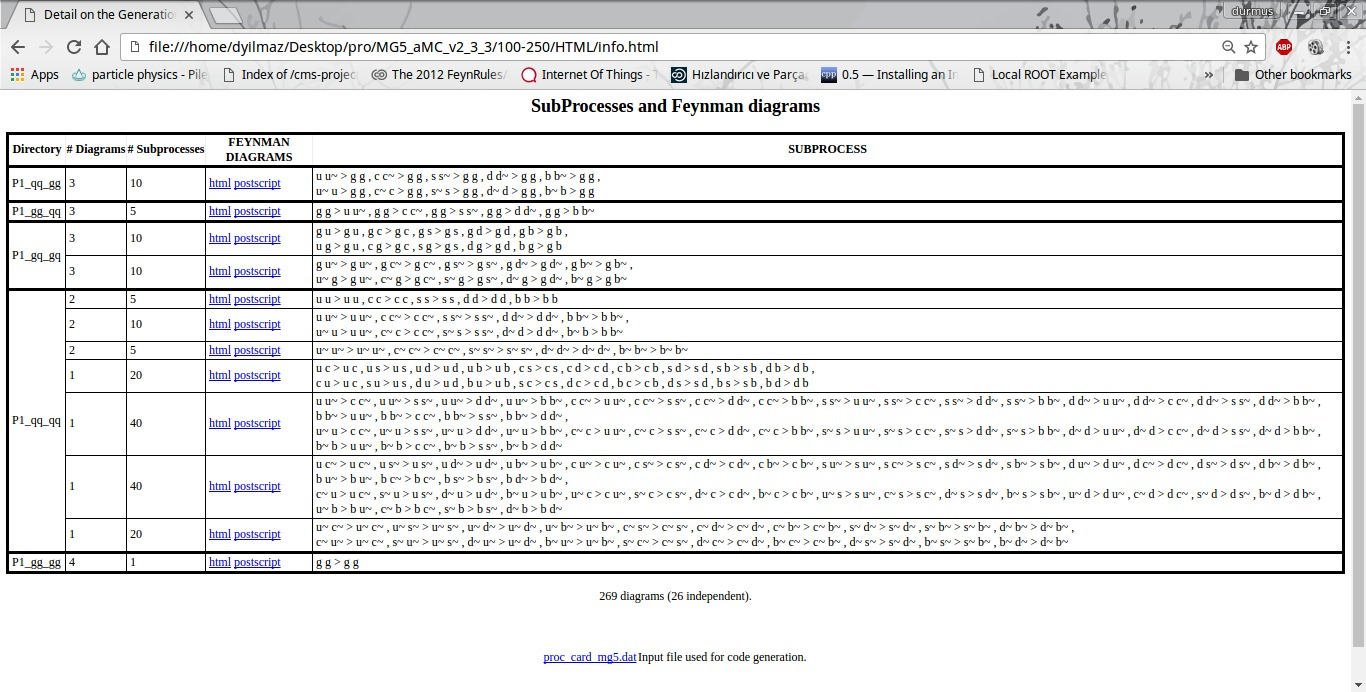
\includegraphics[scale=0.3]{feynrules}
		\caption[p p $>$ j j olayında SM e gore çıkarılan feynman diyagramları]%
        {{\small p p $>$ j j olayında SM e gore çıkarılan feynman diyagramları}}    
        \label{fig:feynrules}
\end{figure}
\par Yüksek Enerji Fiziğinde similasyon için PDG\footnote{PARTICLE NUMBERING SCHEME}(parçacık numaralandırma şeması) 'nın önemli bir yeri vardir. 
Tablo \ref{tab:pdg} bazı önemli parçacıkların PDG leri mevcuttur.\footnote{http://pdg.lbl.gov/2007/reviews/montecarlorpp.pdf}\\
\begin{table}[!htbp]

\centering

\begin{tabular}{|c|c|}

\hline 
\multicolumn{2}{|c|}{Kuarklar} \\ 
\hline 
$d$ & 1 \\ 
\hline 
$u$ & 2 \\ 
\hline 
$s$ & 3 \\ 
\hline 
$c$ & 4 \\ 
\hline 
$b$ & 5 \\ 
\hline 
$t$ & 6 \\ 
\hline 
$b^`$ & 7 \\ 
\hline 
$t^`$ & 8 \\ 
\hline 

\end{tabular} 
\begin{tabular}{|c|c|}

\hline 
\multicolumn{2}{|c|}{Leptonlar} \\ 
\hline 
&\\
\hline 
$e^-$ & 11 \\
\hline 
$\nu_e$ & 12 \\
\hline 
$\mu ^-$ & 13 \\
\hline 
$\nu_\mu$ & 14 \\
\hline 
$\tau^-$ & 15 \\
\hline 
$\nu^\tau$ & 16 \\ 
\hline 

&\\

\hline
\end{tabular}
\begin{tabular}{|c|c|}
\hline 
\multicolumn{2}{|c|}{Bozonlar} \\ 
\hline 
&\\
\hline 
g & 21 \\ 
\hline 
$\gamma$ & 22 \\ 
\hline 
Z & 23 \\ 
\hline 
W & 24 \\ 
\hline 
$h^0 / H^0 $ & 25 \\ 
\hline 
$H^+$ & 37 \\
\hline 
&\\ 
\hline 
\end{tabular} 
\caption{Standart Model deki parçacıkları için PDG kodları}
\label{tab:pdg}
\end{table}


\begin{figure}
\centering
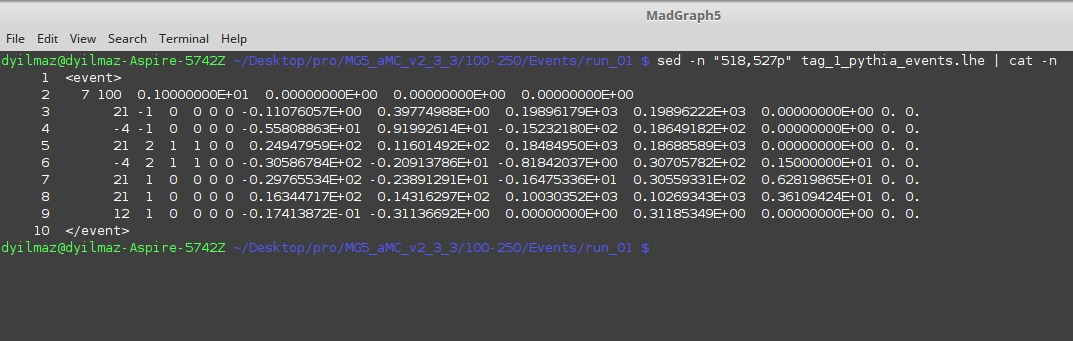
\includegraphics[scale=0.3]{madevent}
\caption{MadEvent çıktı dosyası. İlk satırda çıkan parçacıkların PDG kodları 2. satır başlangıç (-1) son (1) araparçacık (2) bilgisini verir. Ayrıca dört-momuntum ve spin bilgilerinde bu dosyanın içinde mevcuttur.}
\end{figure}

\par \textbf{Pythia}
\par Bu adımda sert saçılma sonrasında parton-duşu\footnote{Parton-Shower} ve hadronizayson yapılmaktadır.Olay üretimimiz sırasında $pythia\_card.dat$ dosyasını kullanmaktadır. Ptyhia gerekli işlemleri yaptıktan sonra bize .HEP\footnote{High Energy Physics} uzantılı dosyayı verir. Artik dedektor similasyonuna sokmadan once elimizde istediğimiz olaya ait verileri almış oluyoruz. \\
Eklerde bulunan $pythia\_card.dat$ dosyasında parton duşunu, hadronisazyonu, çoklu etkileşimi ve kullanacağımız PDF setini seçebiliyoruz. Örnek olarak bizim kullandığımız PDF seti; \\
 \texttt{
	!...PDFset if MG set not supported by pythia-pgs package (set in lhapdf5 or higher)
   \\ LHAID= 10041
      }
\par \textbf{Delphes Similasyonu}
\par Delphes similasyonu ürettiğimiz olaylar üzerinden tıpkı bir dedektör similasyonuna sokulmuş gibi bize dedektör çıktılarını vermektedir. Dedektör similasyonunda ürettiğimiz olayları algıçlar ile etkileşmesi sonucu bizim elimize similasyon verilerini root olarak alırız. Delphes similasyonu $delphes\_card\_CMS.tcl$ kartını kullanmaktadır.
\begin{lstlisting}
 # magnetic field
  set Bz 3.8
\end{lstlisting}
kod satırı ile silindirdeki manyetik alanı ayarlayabiliyoruz.
\begin{lstlisting}
 # algorithm: 1 CDFJetClu, 2 MidPoint, 3 SIScone, 4 kt, 5 Cambridge/Aachen, 6 antikt
  set JetAlgorithm 6
  set ParameterR 0.5

  set JetPTMin 20.0
\end{lstlisting}
ile Jet algoritmalarımızı jet lerin yarıçapları ve minimum jet enerjisini ayarlayarak, similasyonumuzu yönledirebiliyoruz.
\begin{figure}[!h]
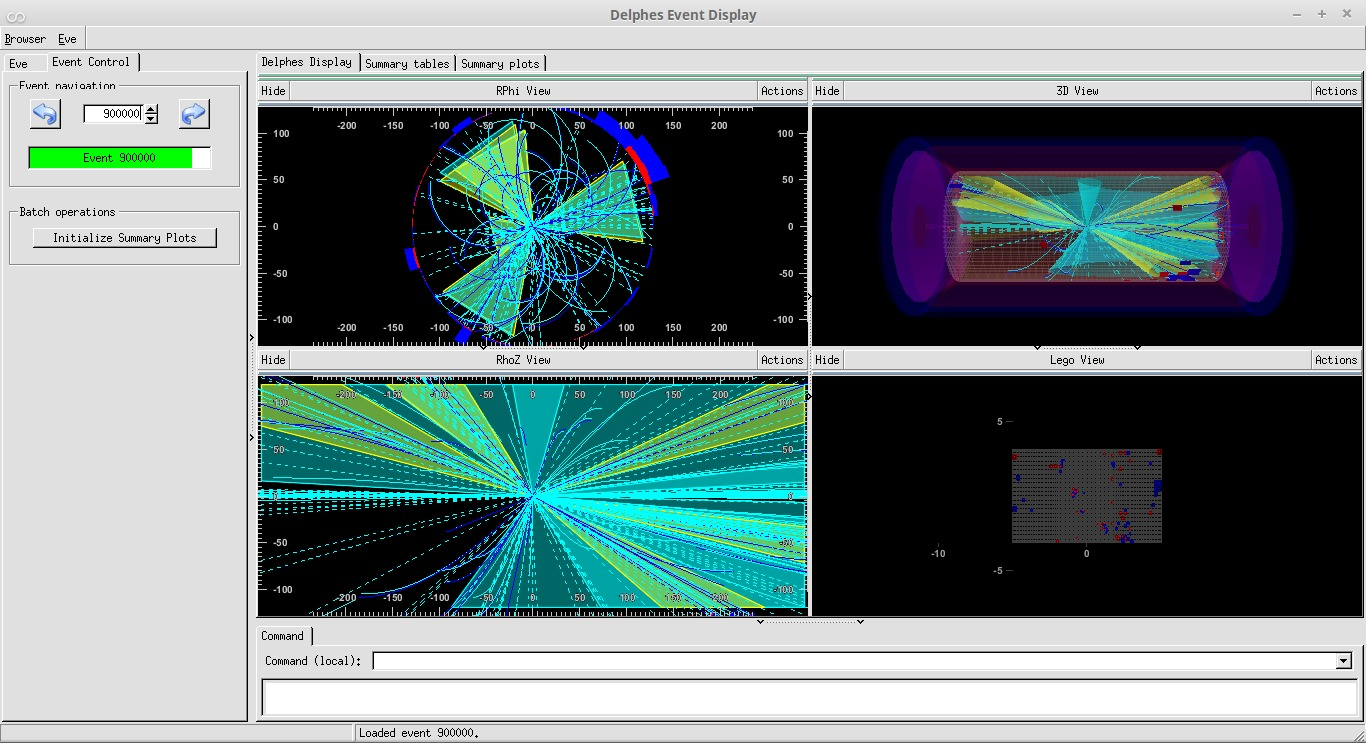
\includegraphics[scale=0.2]{showevent}
\centering
\caption{Delphes Similasyonundan çıkan bir olayın görüntülenmesi}
\label{fig:showevent}
\end{figure}
Şekil \ref{fig:showevent} da göründüğü gibi üretilen bir olayda jetler sınıflandırılmış parçacıklar tanımlanmış ve dedektörün üzerinde hangi parçacığın hangi konumda olduğu hesaplanarak tıpkı gerçek bir olay gibi simüle edilmiş.
\par Deneysel olarak Proton çarpışmasında dedektör üzerine düşen izle hard-disc lere kaylanıyor. Daha sonra bu veriler yeniden yapılandırılarak her bir izin fiziksel karşılığı bulunuyor. Analiz kısmında elde etmiş olduğumuz verilerin histogramları çıkartılıyor. Similasyon kısmında ise MC yöntemş ile yukarıda bahsedilen programlar yardımıyla olaylar simüle ediliyor. Pythia ile dedektör simülasyonundan sonra dedektör üzerindeki izler yeniden yapılandırılıp fiziksel karşılıkları bulunuyor. Analiz kısmında ROOT veya başka bir program ile histogramlar elde ediliyor. Similasyon kısmında teorideki bir model e göre çıkan histogramlar ile deney verisinden eldi edilen veriler karşılaştırılıyor. Eğer deney verisi ile similasyonda farklı sonuçlar verirse teorinin eksik kısımları vardır demek ve düzeltme yapıp tekrardan simülasyon ile deney verileri karşılaştırılıyor. Buna en güzel örnek Standart Model deki Higgs parçacığıdır. Similasyon dan elde edilen veriler ile deneysel veriler karşılaştırıldığında böyle bir parçacığın varlığını ve bu parçacığın özelliklerini tespit edebiliyoruz.



\section{Jet'lerin Yeniden Yapılandırılması ve Algoritmalar}
Kuarklar ve gluon lar renk yüküne sahiptirler({\color{red} r},{\color{green} g},{\color{blue} b}). Kuantum renk dinamiğinin getirdiği kurallardan biri serbest haldeki bir parçacığın renk yükü nötr olmalıdır. Bu yüzden proton-proton çarpışmasında aslında gluon ve kuarkların etkileşmesi incelenirken, serbest halde bulunamayacak olan gluonlar QCD nin izin verdiği müddetçe hadronize olarak kuark antikuark çiftlerine bozulurlar. Böylece bütün renk yükü barındıran parçacıklar hadronizasyon sonucu renksiz parçacıklar oluştururlar.
Jet'ler yüksek enerjili çarpışmalarda açığa çıkan parçacık püskürtüleridir.Kuark ve gluonların dedektörün kalorimetrelerde bıraktıkları enerjilerle tespit edebiliriz. Kısaca parçacık gruplarının oluşturduğu yapıya Jet diyebiliriz. Daha sade bir dil ile söyleyecek olursak jetler yüksek enerji fiziğinde aynı yönde saçılan hadronları tek bir hizaya getirilmiş halleridir. CMS'in yayınladığı araştırmaların $60$ ında Jetler kullanılmıştır. Jetlerin en temel amacı son durumda oluşan karmaşıklığı en aza indirerek basit objeler halinde analiz yapmaktır. Jet algoritmaları için 3 krite vardır. Bunlar collinear güvenilirlik , infrared güvenilirlik ve hız.
\begin{figure}[!htbp]
\centering
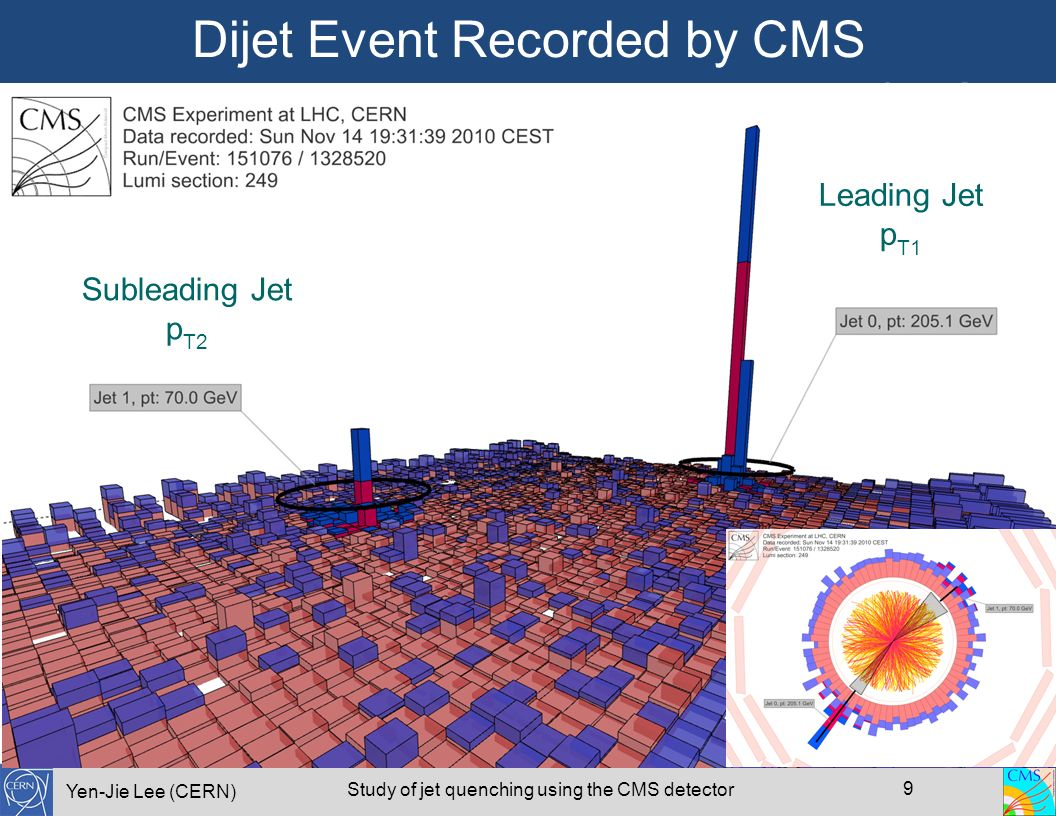
\includegraphics[scale=0.5]{jet}
\caption{2 jet çıkan bir olayın CMS dedektörü üzerindeki izleri}
\label{fig:jet}
\end{figure}

\begin{figure}[!htbp]
\centering


\par Şekil \ref{fig:jet1} de gösterildiği gibi belirlenen bir jet için Jet'in parametreleri;
\begin{equation}
\begin{aligned}
E_{T_{jet}} = \sum_{i \in jet } E_{T_{jet}} \\
\eta_{jet} =\frac{1}{E_{T_{jet}}} \sum_{i \in jet }E_{T_{jet}} \eta_i \\
\phi_{jet} = \frac{1}{E_{T_{jet}}} \sum_{i \in jet }E_{T_{jet}} \phi_i
\end{aligned}
\end{equation}
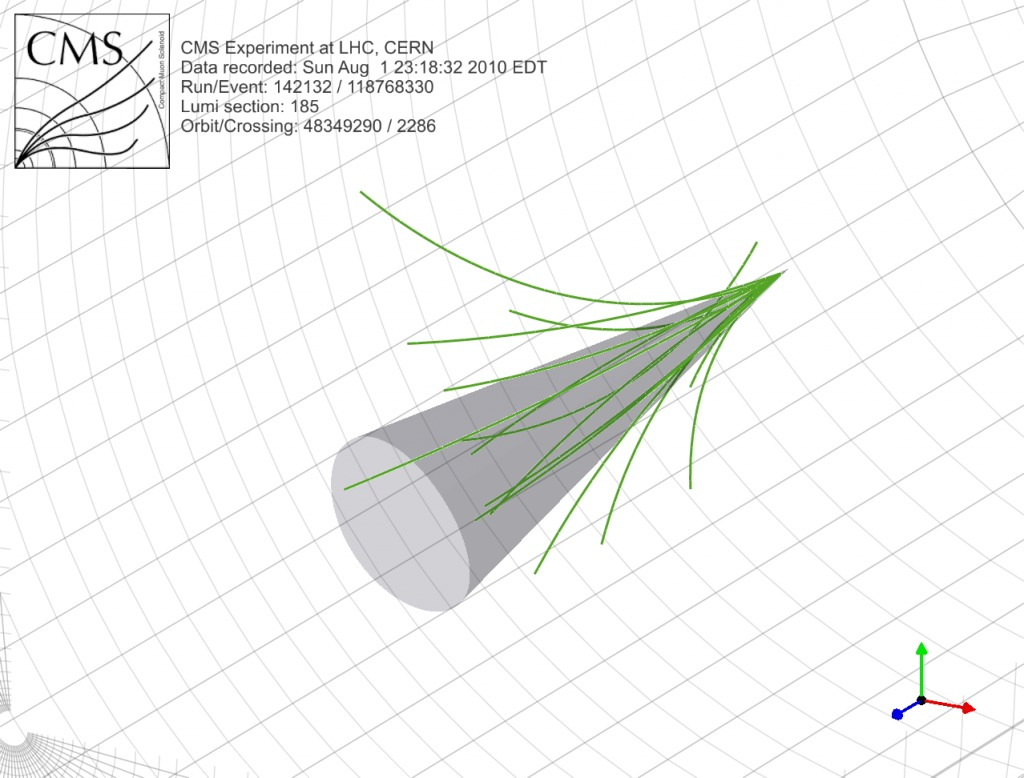
\includegraphics[scale=0.3]{jet1}
\caption{Koni algoritması ile gösterilmiş bir Jet}
\label{fig:jet1}
\end{figure}
\subsection{Jet Algoritmaları}
Temelde iki tip jet algoritma türü vardır. Bunlardan biri koni diğeri kümeleme algoritmasıdır.
\par Koni tipi algoritması kendi içinde 3 e ayrılır. bunlar tekrarlayan koni\footnote{Iterative Cone}  algoritması,  orta nokta \footnote{Midpoint Cone} koni algoritması ve SIS-Cone \footnote{Seedless Infrared-Safe Cone Algorithm}dur. 

\par \textbf{Tekrarlayan koni algoritması} çıkan bütün parçacıkların $p_T$ lerini listeler. Rastgele bir parçacık seçtildikten sonra seçtiğin parçacığın R yarıçaplı bir daire çizerek bu dairenin içinde kalan parçacıkların momentumuna göre tekrar daire çizerek toplar. R yarıçaplı bir dairenin içindeki bütün parçacıkların momentumlarına göre yeniden R yarıçapı çizilerek jet belirlenir.
\begin{figure}[!htbp]
\centering
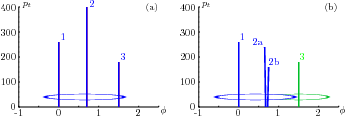
\includegraphics[scale=1]{iterative.png}
\caption{Tekrarlayan koni algoritması en yüksek enerjiye sahip parçacığı seçerek R yarıçapı çemerin içinde kalan bütün parçacıkları toplar}
\end{figure}

\par \textbf{Orta nokta algoritması}Bu algoritmada rastgele ilk jetler belirlenir. Daha sonra her biri için R yarıçaplı daierel çizilir. Eğer iki ilk-jet üst üste geldiyse ve birinin enerjisi diğerinin enerjisinde $\%50$ daha az ise bu bir Jet olarak alınır. 


\par \textbf{SISCONE} 

\par Oldukça hızlı olan bu algoritma CMS tetiklemede kullanılmaktadır. Ancak collinear ve infrared güvenilir değildir.\footnote{collinear ve infrared güvenilirlik Ekler bölümünde anlatılmıştır.}

\par \textbf{Kümeleme Algoritması}\\
Bütün objeler için beam line a olan uzaklık hesaplanır. 
\begin{equation}
d_i = (E_{T,i})^2 \centerdot D^2
\end{equation}

daha sonra diğer parçacıklarla aralarındaki uzaklık hesaplanır.
\begin{equation}
d_{i,j} = min(p_{Ti}^{2p},p_{T j}^{2 p})\frac{\bigtriangleup R_{ij}^2}{R^2}
\end{equation}

\begin{equation}
\bigtriangleup R_{ij}= \sqrt{(y_i-y_j)^2 + (\phi_i - \phi_j)^2} < R
\end{equation}

\par $p=1$ $k_T$ , $p=0$ $Cambridge-Aachen$, $p=-1$ $anti-k_T$ algoritmalarını verir.Tüm parçacıkların birbirinden ve beam-line ndan uzaklıkları belirlenir. Eğer $d_{ij}$ en küçük ise, i ve j parçacıkları birleştirilir ve başa dönülür. Eğer $d_{ib}$ en küçük ise , son durumda Jet olarak belirlenir. Bu işlem hiç bir parçacık kalmayıncaya kadar devam eder.\\
\begin{table}[!htbp]
\centering

\begin{tabular}{|c|c|c|}

\hline 
$k_T$ & $d_{i,j} = min(p_{Ti}^{2p},p_{T j}^{2 p})\frac{\bigtriangleup R_{ij}^2}{R^2}$ & Catani et al ‘91
Ellis, Soper ‘93 \\ 
\hline 
$Cambridge/
Aachen$ & $\frac{\bigtriangleup R_{ij}^2}{R^2}$ & Dokshitzer et al ‘97
Wengler, Wobish ‘98 \\ 
\hline 
$anti-k_T$ & $d_{i,j} = min(p_{Ti}^{2p},p_{T j}^{2 p})\frac{\bigtriangleup R_{ij}^2}{R^2}$ & MC, Salam, Soyez ’08 \\ 
\hline 

\end{tabular} 
\caption{Koni algoritmaları; 2 parçacığın arasındaki mesafe hesabı ve kimin tarafından hangi tarihte yazıldığı}
\end{table}


\begin{figure}
        \centering
        \begin{subfigure}[b]{0.475\textwidth}
            \centering
            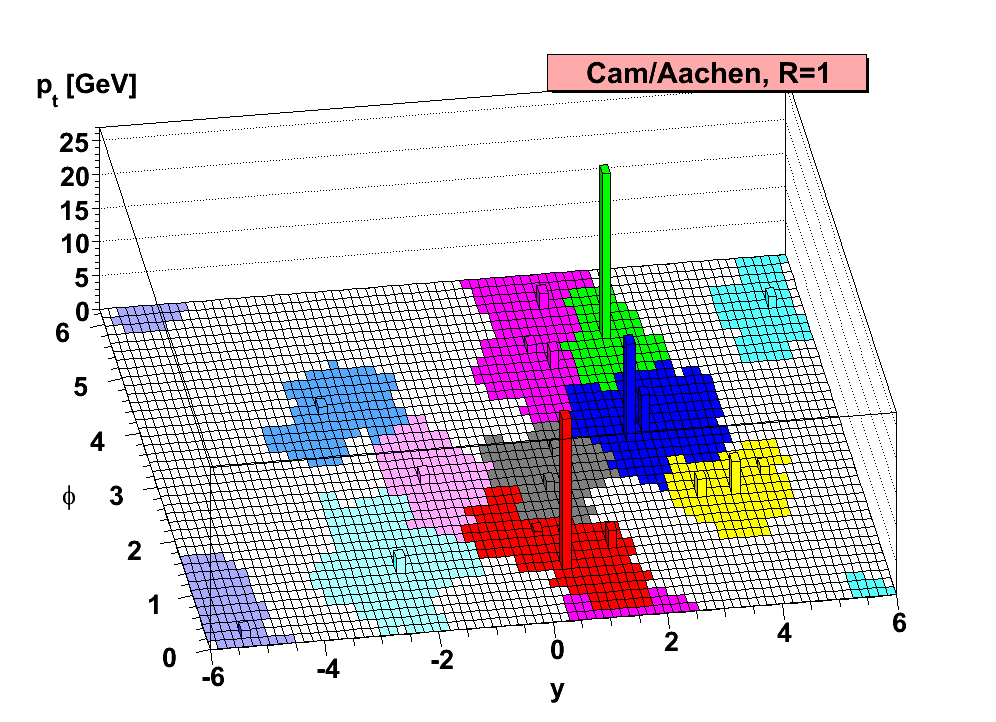
\includegraphics[width=\textwidth]{cam.png}
            \caption[$Cambridge/Aachen$]%
            {{\small $Cambridge/Aachen$}}    
            \label{fig:mean and std of net14}
        \end{subfigure}
        \hfill
        \begin{subfigure}[b]{0.475\textwidth}  
            \centering 
            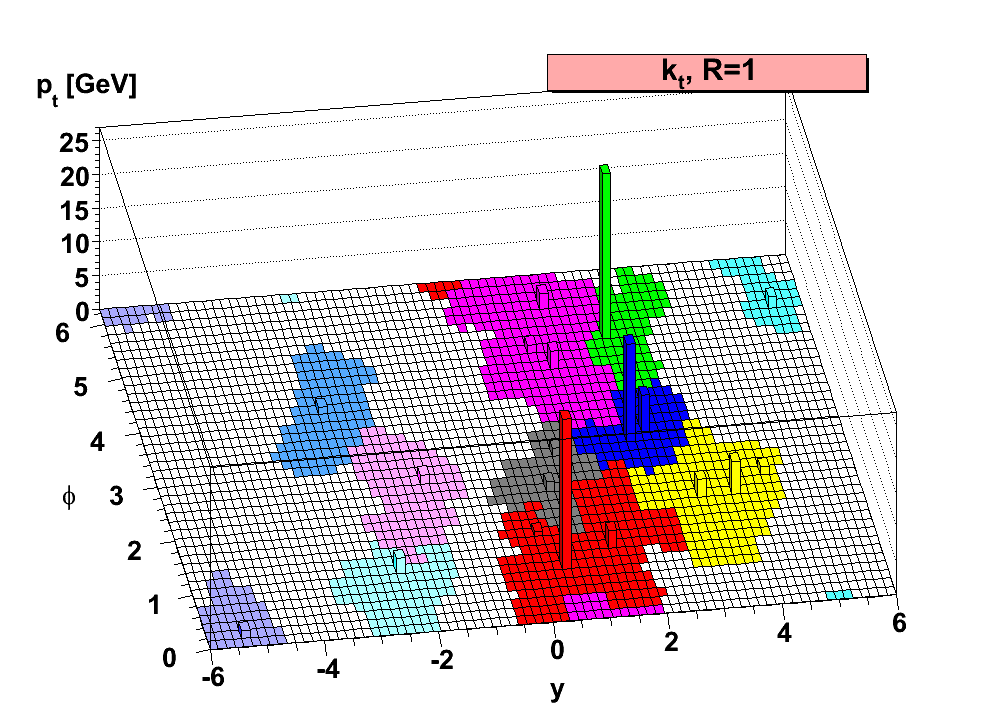
\includegraphics[width=\textwidth]{kt.png}
            \caption[$k_T$ algoritması]%
            {{\small $k_T$ algoritması}}    
            \label{fig:mean and std of net24}
        \end{subfigure}
        \vskip\baselineskip
        \begin{subfigure}[b]{0.475\textwidth}   
            \centering 
            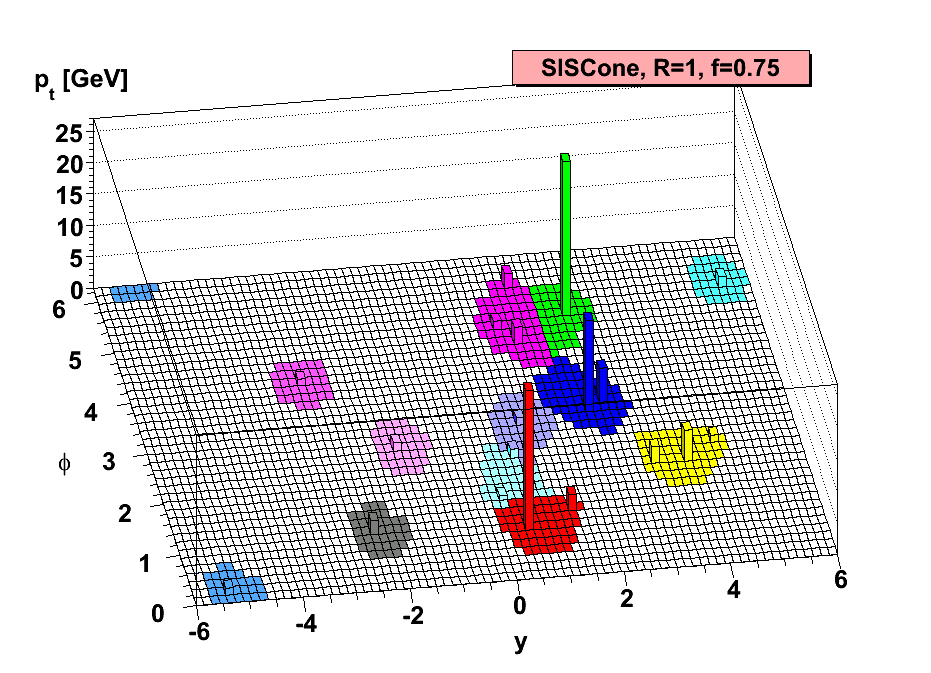
\includegraphics[width=\textwidth]{siscone.png}
            \caption[SISCONE]%
            {{\small SISCONE}}    
            \label{fig:mean and std of net34}
        \end{subfigure}
        \quad
        \begin{subfigure}[b]{0.475\textwidth}   
            \centering 
            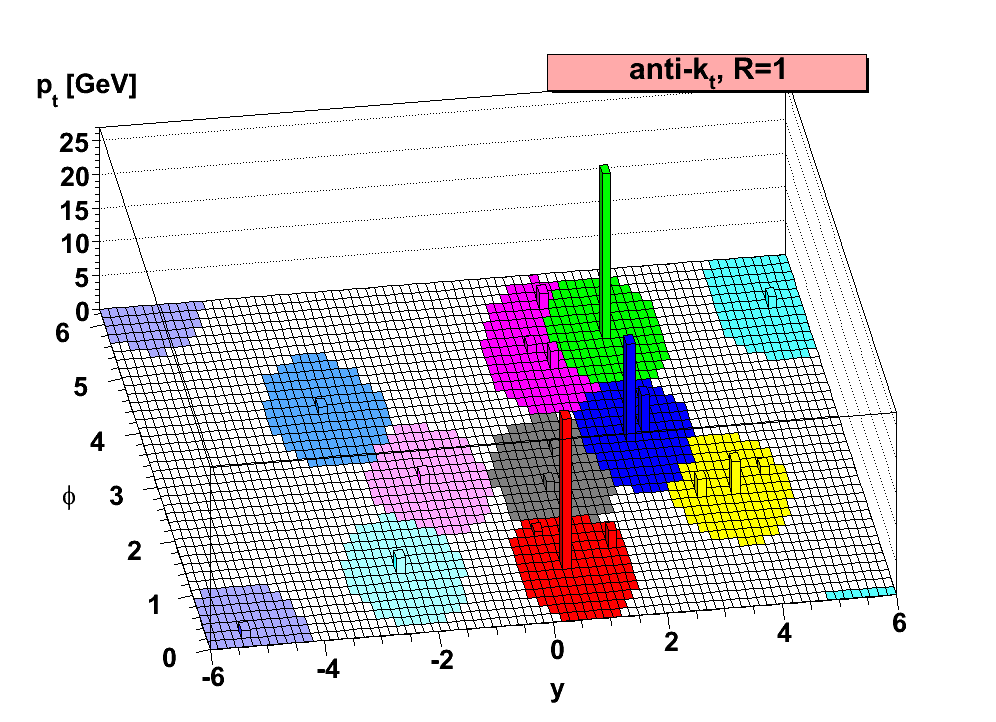
\includegraphics[width=\textwidth]{antikt.png}
            \caption[$anti k_T$]%
            {{\small $anti k_T$}}    
            \label{fig:mean and std of net44}
        \end{subfigure}
        \caption[ 4 farklı Jet algoritmasının parçacıkları sınıflandırması]
        {\small 4 farklı Jet algoritmasının parçacıkları sınıflandırması} 
        \label{fig:jetalgorithm}
    \end{figure}
\section{Datanın Doğrulanması}
\newpage
\chapter{Sonuçlar}
\newpage
\chapter{Ekler}
\section{Bir Oyuncak Kuram Icin Feynman Kurallari}
\begin{center}
\begin{figure}[!ph]
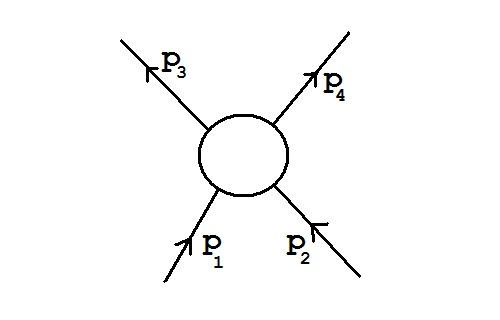
\includegraphics[scale=0.5]{feynmandiagram}
\caption{Dış çizgilerin etiketlendiği bir Feynman diagrami}
\end{figure}
\end{center}
Feynman diyagramına ait $\mathscr{M}$ genliğini bulmak icin Feynman kuralları.
\begin{enumerate}
\item \textbf{Notasyon :} Gelen ve çıkan dört-momentumları, $p_1,p_2,\cdots,p_n$ şeklinde iç momentumları, $q_1,q_2,\cdots$ şeklinde etiketleyin. Herbir çizginin yanında 'pozitif' yönü takip etmek için bir ok çizin (dış çizgiler için zamanda ileriye doğru, iç çizgiler için keyfi yönde).
\item \textbf{Köşe Faktörleri :} Her köşe için, bir
\begin{equation}
-ig
\end{equation}
faktöru yazın. $g$ \textit{çiftlenim sabiti} olarak adlandırılır. A, B, C arasındaki etkileşme şiddetini belirtir. Bu oyuncak kuramda $g$ momentum boyutundadır.
\item \textbf{Propagator :} Her bir çizgi için, bir
\begin{equation}
\frac{i}{q_j^2-m_j^2c^2}
\end{equation}
faktöru yazın. Burada $q_j$, çizginin dört-momentumunu ve $m_j$,çizgisinin betimlediği parçacığın kütlesidir.( $q_j\ neq  m_j^2c^2$ olduğuna dikkat edilmeli, çünkü sanal parçacık kütle kabuğu üzerinde değildir.)
\item \textbf{Enerji ve momentumun korunumu : } Her köşe için, aşağıdaki formda bir delta fonksiyonu yazın.
\begin{equation}
(2 \pi)^2 \delta^4(k_1+k_2+k_3)
\end{equation}
burada $k$'lar köşeye giren üç adet dört-momentumdur.(ok dışa doğru yönelmiş ise $k$ o çizginin dört-momentumunun eksi işaretlisidir). Bu faktör her köşede enerji ve momentum korunumunu zorunlu kılar, çünkü giren momentumların toplamı çıkan momentumlarının toplamına eşit değilse delta fonksiyonu sıfırdır.
\item \textbf{İç momentumlar üzerinde integral alma :} Her bir çizgi için aşağıdaki faktör yazılır.
\begin{equation}
\frac{1}{(2\pi)^4}d^4q_j
\end{equation}
ve tüm iç momentumlar üzerinden integral alınır.
\item \textbf{Delta fonksiyonunun iptali : } Sonuç ,
\begin{equation}
(2\pi)^4 \delta^4(p_1 +p_2+\cdots -p_n)
\end{equation}
şeklinde toplam enerji ve momentumun korunumunu yansıtan bir delta fonksiyonu içerir. Bu faktörü silip ve $i$ ile çarparsak,  sonuç.$\mathscr{M}$ yi verir.
\end{enumerate}
\section{MadGraph5 Kurulumu}
MadGraph\footnote{http://madgraph.phys.ucl.ac.be/} indirildikten sonra;
\begin{enumerate}
\item Sıkıştırılmıştır durumdan çıkartırılır.
\item Çıkartılan dosyanın içerisine terminalden girilir;\\
cd MG5\_ v\_****
\item  Gerekli programlar kurulur \\
MG5\_ aMC $>$ install pythia-pgs \\
MG5\_ aMC $>$ install ExRootAnalysis \\
MG5\_ aMC $>$ install MadAnalysis \\
MG5\_ aMC $>$ install Delphes 
\item Kurulumlar bittikten sonra MadGraph ile olay üretimine baslayabilirsiniz.
\end{enumerate}
\section{Olay Uretimi}
\subsection{Server Uzerinde Olay Uretimi}
Olaylarımızı server üzerinde gerçeklestirirken Shell Script kullandık. Bu bizim için kolaylık sağlamasının yanında zaman kazandırdı. İlgili Shell-script dosyası;

\begin{lstlisting}[language=bash,caption={Feynman diyagramlari ciziliyor}]
#!/bin/bash
echo "====================================="
echo "Start time   : `date`"
echo "====================================="
mg5=~/MG5_aMC_v2_3_3
myfilename="100-250 250-500 500-1000 1000-2500 2500-4000 4000-6000 6000-Inf"
min=(100 250 500 1000 2500 4000 6000)
max=(250 500 1000 2500 4000 6000 100000)
counter=0
for say in $myfilename
do
	cd ${mg5}
	sed -i '/output [a-z]*/c\output '"$say"'' ${mg5}/proc_card.dat
	cd ${mg5}
	./bin/mg5_aMC proc_card.dat
	sed -i '/ 0.0   = htjmin ! minimum jet HT=Sum(jet pt)/c\ '${min[$counter]}'   = htjmin ! minimum jet HT=Sum(jet pt)' ${mg5}/$say/Cards/run_card.dat
	sed -i '/ -1.0  = htjmax ! maximum jet HT=Sum(jet pt)/c\ '${max[$counter]}'   = htjmax ! maximum jet HT=Sum(jet pt)' ${mg5}/$say/Cards/run_card.dat
	sed -i '/ 0.0   = htjmin ! minimum jet HT=Sum(jet pt)/c\ '${min[$counter]}'   = htjmin ! minimum jet HT=Sum(jet pt)' ${mg5}/$say/Cards/run_card_default.dat
	sed -i '/ -1.0  = htjmax ! maximum jet HT=Sum(jet pt)/c\ '${max[$counter]}'   = htjmax ! maximum jet HT=Sum(jet pt)' ${mg5}/$say/Cards/run_card_default.dat
	counter=$((counter+1))
done
cd $mg5
./subrun1.sh
\end{lstlisting}
Burada olay Feynman diyagramlarını çizdiriyoruz. HT\footnote{Enerjisi}' sini istediğimiz aralıklarda tanımlayarak output dosyalarımızı HT aralıklarına göre alıyoruz.

\begin{lstlisting}[language=bash,caption={olay sayisi ayarlaniyor}]
#!/bin/bash

echo "====================================="
echo "Start time   : `date`"
echo "====================================="

#########################################

mg5=~/v2_3_0/MG5_aMC_v2_3_3
myfilename="100-250 250-500 500-1000 1000-2500 2500-4000 4000-6000 6000-Inf"
for say in $myfilename
do
sed -i '/  10000 = nevents ! Number of unweighted events requested/c\  100000 = nevents ! Number of unweighted events requested' ${mg5}/$say/Cards/run_card.dat
sed -i '/  10000 = nevents ! Number of unweighted events requested/c\  100000 = nevents ! Number of unweighted events requested' ${mg5}/$say/Cards/run_card_default.dat
done
cd $mg5
./subrun2.sh
exit 0
\end{lstlisting}
Burada olay sayısını 10000 den 100000 e ayarlıyoruz.

\begin{lstlisting}[language=bash,caption={olaylar uretiliyor}]
#!/bin/bash
mg5=~/MG5_aMC_v2_3_3
myfilename="100-250 250-500 500-1000 1000-2500 2500-4000 4000-6000 6000-Inf"
num_event=5
for say in $myfilename
do
cd ${mg5}/$say
./bin/madevent multi_run $num_event -f --laststep=pythia
done
exit 0
\end{lstlisting}

Artık son olarak Feynman diyagramlarını verdiğimiz olaya göre hesaplandırılması yapılıyor.

\begin{lstlisting}[language=bash,caption={dedektor similasyonu yapiliyor}]
#!/bin/bash
durmusmg5=/home/dyilmaz/tezAnaliz/analiz_1_pp_jj_jjj_jjjj/data
delphes=/home/dyilmaz/v2_3_0/MG5_aMC_v2_3_3/Delphes
HTbins="100-250 250-500 500-1000 1000-2500 2500-4000 4000-6000 6000-Inf"
	for ht in $HTbins # loop over all HTbin directories
	do
		mkdir $delphes/roots_for_$ht
		cd $durmusmg5/$ht/Events 
		for (( i=0 ; i < 5 ; ++i)) ;
		do
			cd run_01_$i
			gunzip tag_1_pythia_events.hep.gz # unzipping the generated hep files
			cd ..
		done
		cd $delphes
		for (( i=0 ; i < 5 ; ++i)) ;
		do
		./DelphesSTDHEP \
			$delphes/cards/delphes_card_CMS.tcl \
			$delphes/roots_for_$ht/run_01_$i.root \
			$durmusmg5/$ht/Events/run_01_$i/tag_1_pythia_events.hep 		done
		cd $delphes/roots_for_$ht
		hadd combined_$ht.root run_01_*.root
	done
exit 0

\end{lstlisting}

Burada hesaplanan Feynman diyagramları ve elde etmiş olduğumuz .hep\footnote{High Energy Physics} uzantılı dosyaları sıkıştırılmış halden çıkartıp delphes\_card\_CMS.tcl kartını kullanarak dedektor similasyonuna sokuyoruz. Bu işlemin sonucunda ürettiğimiz olaylar ROOT programında analiz etmek icin hazır hale geliyor.
\section{Olay Uretiminde kullanilan Kartlar} 
\begin{enumerate}


\item \textbf{proc\_card.dat}

\begin{lstlisting}
#************************************************************
#*                     MadGraph5_aMC@NLO                    *
#*                                                          *
#*                *                       *                 *
#*                  *        * *        *                   *
#*                    * * * * 5 * * * *                     *
#*                  *        * *        *                   *
#*                *                       *                 *
#*                                                          *
#*                                                          *
#*         VERSION 2.2.2                 2014-11-06         *
#*                                                          *
#*    The MadGraph5_aMC@NLO Development Team - Find us at   *
#*    https://server06.fynu.ucl.ac.be/projects/madgraph     *
#*                                                          *
#************************************************************
#*                                                          *
#*               Command File for MadGraph5_aMC@NLO         *
#*                                                          *
#*     run as ./bin/mg5_aMC  filename                       *
#*                                                          *
#************************************************************
set group_subprocesses Auto
set ignore_six_quark_processes False
set gauge unitary
set complex_mass_scheme False
import model sm-no_b_mass
define p = g u c d s u~ c~ d~ s~
define j = g u c d s u~ c~ d~ s~
define l+ = e+ mu+
define l- = e- mu-
define vl = ve vm vt
define vl~ = ve~ vm~ vt~
define p = u c s d b u~ c~ s~ d~ b~ g
define j = u c s d b u~ c~ s~ d~ b~ g
define l = e+ e- mu+ mu- ta+ ta-
generate p p > j j @0
add process p p > j j j @1
add process p p > j j j j @2
output 6000-Inf
\end{lstlisting}
\item \textbf{param\_card.dat}
\begin{lstlisting}
######################################################################
## PARAM_CARD AUTOMATICALY GENERATED BY MG5 FOLLOWING UFO MODEL   ####
######################################################################
##                                                                  ##
##  Width set on Auto will be computed following the information    ##
##        present in the decay.py files of the model.               ##
##        See  arXiv:1402.1178 for more details.                    ##
##                                                                  ##
######################################################################

###################################
## INFORMATION FOR MASS
###################################
Block mass 
    6 1.730000e+02 # MT 
   15 1.777000e+00 # MTA 
   23 9.118800e+01 # MZ 
   25 1.250000e+02 # MH 
## Dependent parameters, given by model restrictions.
## Those values should be edited following the 
## analytical expression. MG5 ignores those values 
## but they are important for interfacing the output of MG5
## to external program such as Pythia.
  1 0.000000 # d : 0.0 
  2 0.000000 # u : 0.0 
  3 0.000000 # s : 0.0 
  4 0.000000 # c : 0.0 
  5 0.000000 # b : 0.0 
  11 0.000000 # e- : 0.0 
  12 0.000000 # ve : 0.0 
  13 0.000000 # mu- : 0.0 
  14 0.000000 # vm : 0.0 
  16 0.000000 # vt : 0.0 
  21 0.000000 # g : 0.0 
  22 0.000000 # a : 0.0 
  24 80.419002 # w+ : cmath.sqrt(MZ__exp__2/2. + cmath.sqrt(MZ__exp__4/4. - (aEW*cmath.pi*MZ__exp__2)/(Gf*sqrt__2))) 

###################################
## INFORMATION FOR SMINPUTS
###################################
Block sminputs 
    1 1.325070e+02 # aEWM1 
    2 1.166390e-05 # Gf 
    3 1.180000e-01 # aS 

###################################
## INFORMATION FOR YUKAWA
###################################
Block yukawa 
    6 1.730000e+02 # ymt 
   15 1.777000e+00 # ymtau 

###################################
## INFORMATION FOR DECAY
###################################
DECAY   6 1.491500e+00 # WT 
DECAY  23 2.441404e+00 # WZ 
DECAY  24 2.047600e+00 # WW 
DECAY  25 6.382339e-03 # WH 
## Dependent parameters, given by model restrictions.
## Those values should be edited following the 
## analytical expression. MG5 ignores those values 
## but they are important for interfacing the output of MG5
## to external program such as Pythia.
DECAY  1 0.000000 # d : 0.0 
DECAY  2 0.000000 # u : 0.0 
DECAY  3 0.000000 # s : 0.0 
DECAY  4 0.000000 # c : 0.0 
DECAY  5 0.000000 # b : 0.0 
DECAY  11 0.000000 # e- : 0.0 
DECAY  12 0.000000 # ve : 0.0 
DECAY  13 0.000000 # mu- : 0.0 
DECAY  14 0.000000 # vm : 0.0 
DECAY  15 0.000000 # ta- : 0.0 
DECAY  16 0.000000 # vt : 0.0 
DECAY  21 0.000000 # g : 0.0 
DECAY  22 0.000000 # a : 0.0 
\end{lstlisting}
\item \textbf{run\_card.dat}
\begin{lstlisting}
#*********************************************************************
#                       MadGraph5_aMC@NLO                            *
#                                                                    *
#                     run_card.dat MadEvent                          *
#                                                                    *
#  This file is used to set the parameters of the run.               *
#                                                                    *
#  Some notation/conventions:                                        *
#                                                                    *
#   Lines starting with a '# ' are info or comments                  *
#                                                                    *
#   mind the format:   value    = variable     ! comment             *
#*********************************************************************
#
#*******************                                                 
# Running parameters
#*******************                                                 
#                                                                    
#*********************************************************************
# Tag name for the run (one word)                                    *
#*********************************************************************
  tag_1     = run_tag ! name of the run 
#*********************************************************************
# Run to generate the grid pack                                      *
#*********************************************************************
  False     = gridpack  !True = setting up the grid pack
#*********************************************************************
# Number of events and rnd seed                                      *
# Warning: Do not generate more than 1M events in a single run       *
# If you want to run Pythia, avoid more than 50k events in a run.    *
#*********************************************************************
  100000 = nevents ! Number of unweighted events requested
  0   = iseed   ! rnd seed (0=assigned automatically=default))
#*********************************************************************
# Collider type and energy                                           *
# lpp: 0=No PDF, 1=proton, -1=antiproton, 2=photon from proton,      *
#                                         3=photon from electron     *
#*********************************************************************
     1        = lpp1    ! beam 1 type 
     1        = lpp2    ! beam 2 type
     6500.0     = ebeam1  ! beam 1 total energy in GeV
     6500.0     = ebeam2  ! beam 2 total energy in GeV
#*********************************************************************
# Beam polarization from -100 (left-handed) to 100 (right-handed)    *
#*********************************************************************
     0.0     = polbeam1 ! beam polarization for beam 1
     0.0     = polbeam2 ! beam polarization for beam 2
#*********************************************************************
# PDF CHOICE: this automatically fixes also alpha_s and its evol.    *
#*********************************************************************
     nn23lo1    = pdlabel     ! PDF set                                     
     230000    = lhaid     ! if pdlabel=lhapdf, this is the lhapdf number
#*********************************************************************
# Renormalization and factorization scales                           *
#*********************************************************************
 False = fixed_ren_scale  ! if .true. use fixed ren scale
 False        = fixed_fac_scale  ! if .true. use fixed fac scale
 91.188  = scale            ! fixed ren scale
 91.188  = dsqrt_q2fact1    ! fixed fact scale for pdf1
 91.188  = dsqrt_q2fact2    ! fixed fact scale for pdf2
 -1 = dynamical_scale_choice ! Choose one of the preselected dynamical choices
 1.0  = scalefact        ! scale factor for event-by-event scales
#*********************************************************************
# Time of flight information. (-1 means not run)
#*********************************************************************
 -1.0 = time_of_flight ! threshold below which info is not written
#*********************************************************************
# Matching - Warning! ickkw > 1 is still beta
#*********************************************************************
 1 = ickkw            ! 0 no matching, 1 MLM, 2 CKKW matching
 1 = highestmult      ! for ickkw=2, highest mult group
 1 = ktscheme         ! for ickkw=1, 1 Durham kT, 2 Pythia pTE
 1.0 = alpsfact         ! scale factor for QCD emission vx
 False = chcluster        ! cluster only according to channel diag
 True = pdfwgt           ! for ickkw=1, perform pdf reweighting
 5 = asrwgtflavor     ! highest quark flavor for a_s reweight
 True = clusinfo         ! include clustering tag in output
 3.0 = lhe_version       ! Change the way clustering information pass to shower.        
#*********************************************************************
#**********************************************************
#
#**********************************************************
# Automatic ptj and mjj cuts if xqcut > 0
# (turn off for VBF and single top processes)
#**********************************************************
   True  = auto_ptj_mjj  ! Automatic setting of ptj and mjj
#**********************************************************
#                                                                    
#**********************************
# BW cutoff (M+/-bwcutoff*Gamma)
#**********************************
  15.0  = bwcutoff      ! (M+/-bwcutoff*Gamma)
#**********************************************************
# Apply pt/E/eta/dr/mij/kt_durham cuts on decay products or not
# (note that etmiss/ptll/ptheavy/ht/sorted cuts always apply)
#*************************************************************
   False  = cut_decays    ! Cut decay products 
#*************************************************************
# Number of helicities to sum per event (0 = all helicities)
# 0 gives more stable result, but longer run time (needed for
# long decay chains e.g.).
# Use >=2 if most helicities contribute, e.g. pure QCD.
#*************************************************************
   0  = nhel          ! Number of helicities used per event
#*******************                                                 
# Standard Cuts
#*******************                                                 
#                                                                    
#*********************************************************************
# Minimum and maximum pt's (for max, -1 means no cut)                *
#*********************************************************************
 20.0  = ptj       ! minimum pt for the jets 
 0.0  = ptb       ! minimum pt for the b 
 10.0  = pta       ! minimum pt for the photons 
 10.0  = ptl       ! minimum pt for the charged leptons 
 0.0  = misset    ! minimum missing Et (sum of neutrino's momenta)
 0.0  = ptheavy   ! minimum pt for one heavy final state
 -1.0  = ptjmax    ! maximum pt for the jets
 -1.0  = ptbmax    ! maximum pt for the b
 -1.0  = ptamax    ! maximum pt for the photons
 -1.0  = ptlmax    ! maximum pt for the charged leptons
 -1.0  = missetmax ! maximum missing Et (sum of neutrino's momenta)
#*********************************************************************
# Minimum and maximum E's (in the center of mass frame)              *
#*********************************************************************
  0.0  = ej     ! minimum E for the jets 
  0.0  = eb     ! minimum E for the b 
  0.0  = ea     ! minimum E for the photons 
  0.0  = el     ! minimum E for the charged leptons 
  -1.0   = ejmax ! maximum E for the jets
 -1.0   = ebmax ! maximum E for the b
 -1.0   = eamax ! maximum E for the photons
 -1.0   = elmax ! maximum E for the charged leptons
#*********************************************************************
# Maximum and minimum absolute rapidity (for max, -1 means no cut)   *
#*********************************************************************
  5.0 = etaj    ! max rap for the jets 
  -1.0  = etab    ! max rap for the b
 2.5  = etaa    ! max rap for the photons 
 2.5  = etal    ! max rap for the charged leptons 
 0.0  = etajmin ! min rap for the jets
 0.0  = etabmin ! min rap for the b
 0.0  = etaamin ! min rap for the photons
 0.0  = etalmin ! main rap for the charged leptons
#*********************************************************************
# Minimum and maximum DeltaR distance                                *
#*********************************************************************
 0.0 = drjj    ! min distance between jets 
 0.0   = drbb    ! min distance between b's 
 0.4 = drll    ! min distance between leptons 
 0.4 = draa    ! min distance between gammas 
 0.0   = drbj    ! min distance between b and jet 
 0.4 = draj    ! min distance between gamma and jet 
 0.0 = drjl    ! min distance between jet and lepton 
 0.0   = drab    ! min distance between gamma and b 
 0.0   = drbl    ! min distance between b and lepton 
 0.4 = dral    ! min distance between gamma and lepton 
 -1.0  = drjjmax ! max distance between jets
 -1.0  = drbbmax ! max distance between b's
 -1.0  = drllmax ! max distance between leptons
 -1.0  = draamax ! max distance between gammas
 -1.0  = drbjmax ! max distance between b and jet
 -1.0  = drajmax ! max distance between gamma and jet
 -1.0  = drjlmax ! max distance between jet and lepton
 -1.0  = drabmax ! max distance between gamma and b
 -1.0  = drblmax ! max distance between b and lepton
 -1.0  = dralmax ! maxdistance between gamma and lepton
#*********************************************************************
# Minimum and maximum invariant mass for pairs                       *
# WARNING: for four lepton final state mmll cut require to have      *
#          different lepton masses for each flavor!                  *           
#*********************************************************************
 0.0   = mmjj    ! min invariant mass of a jet pair 
 0.0   = mmbb    ! min invariant mass of a b pair 
 0.0   = mmaa    ! min invariant mass of gamma gamma pair
 0.0   = mmll    ! min invariant mass of l+l- (same flavour) lepton pair
 -1.0  = mmjjmax ! max invariant mass of a jet pair
 -1.0  = mmbbmax ! max invariant mass of a b pair
 -1.0  = mmaamax ! max invariant mass of gamma gamma pair
 -1.0  = mmllmax ! max invariant mass of l+l- (same flavour) lepton pair
#*********************************************************************
# Minimum and maximum invariant mass for all letpons                 *
#*********************************************************************
 0.0   = mmnl    ! min invariant mass for all letpons (l+- and vl) 
 -1.0  = mmnlmax ! max invariant mass for all letpons (l+- and vl) 
#*********************************************************************
# Minimum and maximum pt for 4-momenta sum of leptons                *
#*********************************************************************
 0.0   = ptllmin  ! Minimum pt for 4-momenta sum of leptons(l and vl)
 -1.0  = ptllmax  ! Maximum pt for 4-momenta sum of leptons(l and vl)
#*********************************************************************
# Inclusive cuts                                                     *
#*********************************************************************
 0.0  = xptj ! minimum pt for at least one jet  
 0.0  = xptb ! minimum pt for at least one b 
 0.0  = xpta ! minimum pt for at least one photon 
 0.0  = xptl ! minimum pt for at least one charged lepton 
#*********************************************************************
# Control the pt's of the jets sorted by pt                          *
#*********************************************************************
 0.0   = ptj1min ! minimum pt for the leading jet in pt
 0.0   = ptj2min ! minimum pt for the second jet in pt
 0.0   = ptj3min ! minimum pt for the third jet in pt
 0.0   = ptj4min ! minimum pt for the fourth jet in pt
 -1.0  = ptj1max ! maximum pt for the leading jet in pt 
 -1.0  = ptj2max ! maximum pt for the second jet in pt
 -1.0  = ptj3max ! maximum pt for the third jet in pt
 -1.0  = ptj4max ! maximum pt for the fourth jet in pt
 0   = cutuse  ! reject event if fails any (0) / all (1) jet pt cuts
#*********************************************************************
# Control the pt's of leptons sorted by pt                           *
#*********************************************************************
 0.0   = ptl1min ! minimum pt for the leading lepton in pt
 0.0   = ptl2min ! minimum pt for the second lepton in pt
 0.0   = ptl3min ! minimum pt for the third lepton in pt
 0.0   = ptl4min ! minimum pt for the fourth lepton in pt
 -1.0  = ptl1max ! maximum pt for the leading lepton in pt 
 -1.0  = ptl2max ! maximum pt for the second lepton in pt
 -1.0  = ptl3max ! maximum pt for the third lepton in pt
 -1.0  = ptl4max ! maximum pt for the fourth lepton in pt
#*********************************************************************
# Control the Ht(k)=Sum of k leading jets                            *
#*********************************************************************
 100   = htjmin ! minimum jet HT=Sum(jet pt)
 250   = htjmax ! maximum jet HT=Sum(jet pt)
 0.0   = ihtmin  !inclusive Ht for all partons (including b)
 -1.0  = ihtmax  !inclusive Ht for all partons (including b)
 0.0   = ht2min ! minimum Ht for the two leading jets
 0.0   = ht3min ! minimum Ht for the three leading jets
 0.0   = ht4min ! minimum Ht for the four leading jets
 -1.0  = ht2max ! maximum Ht for the two leading jets
 -1.0  = ht3max ! maximum Ht for the three leading jets
 -1.0  = ht4max ! maximum Ht for the four leading jets
#***********************************************************************
# Photon-isolation cuts, according to hep-ph/9801442                   *
# When ptgmin=0, all the other parameters are ignored                  *
# When ptgmin>0, pta and draj are not going to be used                 *
#***********************************************************************
 0.0 = ptgmin ! Min photon transverse momentum
 0.4 = R0gamma ! Radius of isolation code
 1.0 = xn ! n parameter of eq.(3.4) in hep-ph/9801442
 1.0 = epsgamma ! epsilon_gamma parameter of eq.(3.4) in hep-ph/9801442
 True = isoEM ! isolate photons from EM energy (photons and leptons)
#*********************************************************************
# WBF cuts                                                           *
#*********************************************************************
 0.0   = xetamin ! minimum rapidity for two jets in the WBF case  
 0.0   = deltaeta ! minimum rapidity for two jets in the WBF case 
#*********************************************************************
# KT DURHAM CUT                                                      *
#*********************************************************************
 -1.0    =  ktdurham        
 0.4  =  dparameter 
#*********************************************************************
# maximal pdg code for quark to be considered as a light jet         *
# (otherwise b cuts are applied)                                     *
#*********************************************************************
 5 = maxjetflavor    ! Maximum jet pdg code
#*********************************************************************
# Jet measure cuts                                                   *
#*********************************************************************
 30.0   = xqcut   ! minimum kt jet measure between partons
#*********************************************************************
#
#*********************************************************************
# Store info for systematics studies                                 *
# WARNING: If use_syst is T, matched Pythia output is                *
#          meaningful ONLY if plotted taking matchscale              *
#          reweighting into account!                                 *
#*********************************************************************
   False  = use_syst      ! Enable systematics studies
#
#**************************************
# Parameter of the systematics study
#  will be used by SysCalc (if installed)
#**************************************                                  
#
0.5 1 2 = sys_scalefact  # factorization/renormalization scale factor
0.5 1 2 = sys_alpsfact  # \alpha_s emission scale factors
30 50 = sys_matchscale # variation of merging scale
# PDF sets and number of members (0 or none for all members).
Ct10nlo.LHgrid = sys_pdf # matching scales
# MSTW2008nlo68cl.LHgrid 1  = sys_pdf
\end{lstlisting}
\item \textbf{pythia\_card.dat}
\begin{lstlisting}
!...Parton showering on or off  
      MSTP(61)=1
      MSTP(71)=1
 
!...Fragmentation/hadronization on or off 
      MSTJ(1)=1
 
!...Multiple interactions on or off 
      MSTP(81)=20 

!...Don't stop execution after 10 errors
      MSTU(21)=1

!...PDFset if MG set not supported by pythia-pgs package (set in lhapdf5 or higher)
      LHAID= 10041

\end{lstlisting}
\item \textbf{pgs\_card\_CMS.dat}
\begin{lstlisting}
CMS                 ! parameter set name
70                  ! eta cells in calorimeter  
70                  ! phi cells in calorimeter
0.087               ! eta width of calorimeter cells  |eta| < 3
0.0897597901        ! phi width of calorimeter cells
0.01                ! electromagnetic calorimeter resolution  const
0.03                ! electromagnetic calorimeter resolution * sqrt(E)
1.25                ! hadronic calolrimeter resolution * sqrt(E)
0.2                 ! MET resolution
0.00                ! calorimeter cell edge crack fraction
cone                ! jet finding algorithm (cone or ktjet)
0.5                 ! calorimeter trigger cluster finding seed threshold (GeV)
0.5                 ! calorimeter trigger cluster finding shoulder threshold (GeV)
0.5                 ! calorimeter kt cluster finder cone size (delta R)
1.1                 ! outer radius of tracker (m)
4.0                 ! magnetic field (T)
0.000020            ! sagitta resolution (m)
0.98                ! track finding efficiency
0.90                ! minimum track pt (GeV/c)
2.4                 ! tracking eta coverage
3.0                 ! e/gamma eta coverage
2.4                 ! muon eta coverage
2.0                 ! tau eta coverage
\end{lstlisting}
\end{enumerate}
\section{Collinear ve Infrared Güvenilirlik}

\begin{wrapfigure}{r}{3cm}
\caption{Infrared ve eş yönlü güvenlilik}
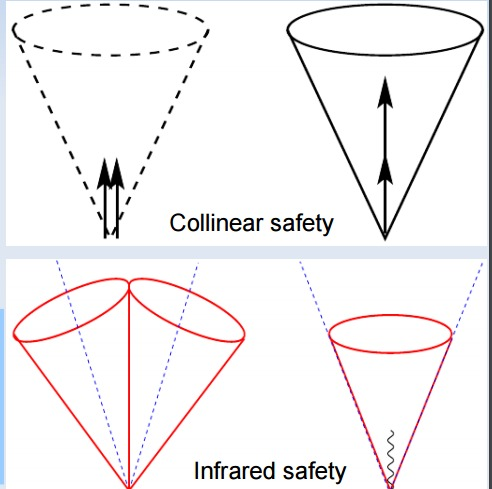
\includegraphics[width=3cm]{safe}
\end{wrapfigure}
Eşyönlü güvenilirlikte çıkan bir partonun yanında neredeyse aynı yönde $\theta = 0$ olacak şekilde başkabir parçacığa bozunuyorsa orada sonsuzluk veriyor ve bu jet yapılandırma algoritmasını bozuyor. Buna eşyönlü güvenilirlik deniliyor. 
Infrared güvenilirlik ise enerjisi çok düşük bir parçacık çıkıyorsa bu yine sonsuzluk meydana getiriyor buna buda tekrardan Jet yapılandırma algoritmasını bozmaktadır. Bu yüzden Jet yapılandırma algoritması hem eşyönlü güvenilir hemde Infrared güvenilir olması gerekmektedir.\\


\begin{thebibliography}{9}

\bibitem{apalike}
  Temel Parçacıklara Giriş - David Griffiths
  
\bibitem{apalike}
	Jet matching and subtraction methods for associated squark-gluino production - Jennifer Kieselmann
\bibitem{apalike}
PYTHIA - AN EVENT GENERATOR - Dr. Hafeez Hoorani

\bibitem{apalike}
MadGraph Tutorial - Olivier Mattelaer

\bibitem{apalike}
Introduction to FeynRules - Claude Duhr

\bibitem{apalike}
The VISION of MadGraph and FeynRules - Johan Alwall

\bibitem{apalike}
MadGraph 5 - Olivier Mattelaer

\bibitem{apalike}
FeynRules/MadGraph aMC@NLO/MadAnalysis5
tutorial - Benj, Claude, Kentarou, Fabio, Marco, Olivier

\bibitem{apalike}
Jet matching and subtraction methods
for associated squark-gluino production - Jennifer Kieselmann

\bibitem{apalike}
Monte Carlo’s:
event simulation for the LHC - Fabio Maltoni

\bibitem{apalike}
Jet quenching in heavy-ion collisions at LHC with
CMS detector - Yetkin YILMAZ

\bibitem{apalike}
Monte Carlo Methods
in High Energy Physics -WIESLAW PLACZEK
\bibitem{apalike}
Jet Yapılandırma ve FastJet Programı - Sertaç Öztürk

\bibitem{apalike}
Performance of Jet Reconstruction
at CMS - On behalf of the CMS collaboration
Christian Sander (University of Hamburg)
\end{thebibliography}


\end{document}